\documentclass[12pt]{article}
\usepackage[utf8]{inputenc}
\usepackage{amsmath,amsthm,amsfonts,amssymb}
\usepackage{tikz}
% \usepackage{subfig}
\usepackage[english]{babel}
\usepackage{capt-of}
\usepackage{tabularray}
\usepackage{caption}
\usepackage{subcaption}
% \usepackage{subcaption}
% \captionsetup{compatibility=false}
\usepackage{graphicx}
\newtheorem{theorem}{Theorem}
\usetikzlibrary{calc}
\usetikzlibrary{shapes}
\usepackage{hyperref}
%might be unnecessary
\usepackage{doi}

%bibliography CMDS

%\usepackage{cite}
%\usepackage[style=alphabetic]{biblatex}
%\bibliographystyle{plain}

%\usepackage[style=alphabetic]{biblatex}

% \usepackage[backend=biber,style=alphabetic]{biblatex}
\usepackage[backend=biber,style=numeric]{biblatex}
% \usepackage[backend=biber,style=abbrv]{biblatex}
% \usepackage[backend=biber,style=alpha]{biblatex}
%\usepackage[backend=bibtex,style=alphabetic]{biblatex}
\addbibresource{./bibb.bib}

%%% With amsthm package, creates environments for nicely formatted,
%%% labeled, and numbered propositions, etc.
\theoremstyle{plain}

\newtheorem{thm}{Theorem}[section]
\newtheorem{lemma}[thm]{Lemma}
\newtheorem{prop}[thm]{Proposition}
\newtheorem{conj}[thm]{Conjecture}
\newtheorem{cor}[thm]{Corollary}
\newtheorem{claim}[thm]{Claim}
\newtheorem{fact}[thm]{Fact}
\newtheorem{constraint}[thm]{Constraint}
\newtheorem{condition}[thm]{Condition}

\theoremstyle{definition}
\newtheorem{eg}[thm]{Example}
% \newtheorem{defn}[thm]{Definition}
\newtheorem{definition}{Definition}[section]
\newtheorem{rem}[thm]{Remark}
\newtheorem{observ}[thm]{Observation}
\newtheorem{open}[thm]{Open Problem}
\newtheorem{prob.}[thm]{Problem}
\newtheorem{quest}[thm]{Question}

% I used these for making definitions and theorems, not what is above
\theoremstyle{remark}
\newtheorem{remark}[thm]{Remark}
\newtheorem{note}[thm]{Note}

\theoremstyle{definition}
% \newtheorem{definition}{Definition}[section]
\newtheorem{exmp}{Example}[section]

%custom commands

% blank cell
\newcommand{\cell}[4]{ \draw[thick] ( #1 , #2 ) rectangle ( #3 , #4 );}

% invisible cell for spacing
\newcommand{\spacecell}[4]{ \draw[thick, color=white] ( #1 , #2 ) rectangle ( #3 , #4 );}

% open cell 
\newcommand{\cellopen}[4]{ \draw[thick] ( #1 , #2 ) rectangle ( #3 , #4 ); \node[shape=circle,draw=red,fill=red, inner sep=0pt,minimum size=3pt] (A) at ( #1 * 0.5 + #3 * 0.5 , #2 * 0.5 + #4 * 0.5 ){};}
% /
% \newcommand{\cellA}[4]{ \draw[thick] ( #1 , #2 ) rectangle ( #3 , #4 ); \draw[red, thick, densely dotted] (#3 * 0.5 + #1 * 0.5 , #2) -- (#3, #4 * 0.5 + #2 * 0.5);}
% \
% \newcommand{\cellB}[4]{ \draw[thick] ( #1 , #2 ) rectangle ( #3 , #4 ); \draw[red, thick, densely dotted] (#3 * 0.5 + #1 * 0.5 , #2) -- (#1, #4 * 0.5 + #2 * 0.5);}
% /
% \newcommand{\cellC}[4]{ \draw[thick] ( #1 , #2 ) rectangle ( #3 , #4 ); \draw[red, thick, densely dotted] (#3 * 0.5 + #1 * 0.5 , #4) -- (#1, #4 * 0.5 + #2 * 0.5);}
% L
% \newcommand{\cellD}[4]{ \draw[thick] ( #1 , #2 ) rectangle ( #3 , #4 ); \draw[red, thick, densely dotted] (#3 * 0.5 + #1 * 0.5 , #4) -- (#3, #4 * 0.5 + #2 * 0.5);}
% |
% \newcommand{\cellE}[4]{ \draw[thick] ( #1 , #2 ) rectangle ( #3 , #4 ); \draw[red, thick, densely dotted] (#3 * 0.5 + #1 * 0.5 , #2) -- (#3 * 0.5 + #1 * 0.5 , #4);}
% % -
% \newcommand{\cellF}[4]{ \draw[thick] ( #1 , #2 ) rectangle ( #3 , #4 ); \draw[red, thick, densely dotted] (#3, #4 * 0.5 + #2 * 0.5) -- (#1, #4 * 0.5 + #2 * 0.5);}

% \newcommand{\cellAf}[4]{\filldraw[gray!40] ( #1 , #2 ) rectangle ( #3 , #4 ); \draw[thick] ( #1 , #2 ) rectangle ( #3 , #4 ); \draw[red, thick, densely dotted] (#3 * 0.5 + #1 * 0.5 , #2) -- (#3, #4 * 0.5 + #2 * 0.5);}
% \
% \newcommand{\cellBf}[4]{\filldraw[gray!40] ( #1 , #2 ) rectangle ( #3 , #4 ); \draw[thick] ( #1 , #2 ) rectangle ( #3 , #4 ); \draw[red, thick, densely dotted] (#3 * 0.5 + #1 * 0.5 , #2) -- (#1, #4 * 0.5 + #2 * 0.5);}
% /
% \newcommand{\cellCf}[4]{\filldraw[gray!40] ( #1 , #2 ) rectangle ( #3 , #4 ); \draw[thick] ( #1 , #2 ) rectangle ( #3 , #4 ); \draw[red, thick, densely dotted] (#3 * 0.5 + #1 * 0.5 , #4) -- (#1, #4 * 0.5 + #2 * 0.5);}
% L
% \newcommand{\cellDf}[4]{\filldraw[gray!40] ( #1 , #2 ) rectangle ( #3 , #4 ); \draw[thick] ( #1 , #2 ) rectangle ( #3 , #4 ); \draw[red, thick, densely dotted] (#3 * 0.5 + #1 * 0.5 , #4) -- (#3, #4 * 0.5 + #2 * 0.5);}
% |
% \newcommand{\cellEf}[4]{\filldraw[gray!40] ( #1 , #2 ) rectangle ( #3 , #4 ); \draw[thick] ( #1 , #2 ) rectangle ( #3 , #4 ); \draw[red, thick, densely dotted] (#3 * 0.5 + #1 * 0.5 , #2) -- (#3 * 0.5 + #1 * 0.5 , #4);}
% % -
% \newcommand{\cellFf}[4]{\filldraw[gray!40] ( #1 , #2 ) rectangle ( #3 , #4 ); \draw[thick] ( #1 , #2 ) rectangle ( #3 , #4 ); \draw[red, thick, densely dotted] (#3, #4 * 0.5 + #2 * 0.5) -- (#1, #4 * 0.5 + #2 * 0.5);}


\newcommand{\cellA}[4]{\draw[red, thick, densely dotted] ( #1 + 0.5 , #2 ) arc(0:90:{0.5}); \draw[thick] ( #1 , #2 ) rectangle ( #3 , #4 );}
\newcommand{\cellB}[4]{\draw[red, thick, densely dotted] ( #1 + 1 , #2 + 0.5 ) arc(90:180:{0.5}); \draw[thick] ( #1 , #2 ) rectangle ( #3 , #4 );}
\newcommand{\cellC}[4]{\draw[red, thick, densely dotted] ( #1 + 0.5, #2 + 1 ) arc(180:270:{0.5}); \draw[thick] ( #1 , #2 ) rectangle ( #3 , #4 );}
\newcommand{\cellD}[4]{\draw[red, thick, densely dotted] ( #1 , #2 + 0.5 ) arc(-90:0:{0.5}); \draw[thick] ( #1 , #2 ) rectangle ( #3 , #4 );}
\newcommand{\cellE}[4]{\draw[red, thick, densely dotted] (#3, #4 * 0.5 + #2 * 0.5) -- (#1, #4 * 0.5 + #2 * 0.5); \draw[thick] ( #1 , #2 ) rectangle ( #3 , #4 );}
\newcommand{\cellF}[4]{\draw[red, thick, densely dotted] (#3 * 0.5 + #1 * 0.5 , #2) -- (#3 * 0.5 + #1 * 0.5 , #4); \draw[thick] ( #1 , #2 ) rectangle ( #3 , #4 );}
\newcommand{\cellG}[4]{\draw[red, thick, densely dotted] ( #1 + 0.5 , #2 ) arc(0:90:{0.5}); \draw[red, thick, densely dotted] ( #1 + 0.5, #2 + 1 ) arc(180:270:{0.5}); \draw[thick] ( #1 , #2 ) rectangle ( #3 , #4 );}
\newcommand{\cellH}[4]{\draw[red, thick, densely dotted] ( #1 , #2 + 0.5 ) arc(-90:0:{0.5}); \draw[red, thick, densely dotted] ( #1 + 1 , #2 + 0.5 ) arc(90:180:{0.5}); \draw[thick] ( #1 , #2 ) rectangle ( #3 , #4 );}
\newcommand{\cellI}[4]{\draw[red, thick, densely dotted] (#3 * 0.5 + #1 * 0.5 , #2) -- (#3 * 0.5 + #1 * 0.5 , #4); \node[shape=circle,draw=none,fill=white, inner sep=3pt,minimum size=5pt] (A) at ( #1 + 0.5 , #2 + 0.5 ) {}; \draw[red, thick, densely dotted] (#3, #4 * 0.5 + #2 * 0.5) -- (#1, #4 * 0.5 + #2 * 0.5); \draw[thick] ( #1 , #2 ) rectangle ( #3 , #4 );}
\newcommand{\cellJ}[4]{\draw[red, thick, densely dotted] (#3, #4 * 0.5 + #2 * 0.5) -- (#1, #4 * 0.5 + #2 * 0.5); \node[shape=circle,draw=none,fill=white, inner sep=3pt,minimum size=5pt] (A) at ( #1 + 0.5 , #2 + 0.5 ) {}; \draw[thick] ( #1 , #2 ) rectangle ( #3 , #4 ); \draw[red, thick, densely dotted] (#3 * 0.5 + #1 * 0.5 , #2) -- (#3 * 0.5 + #1 * 0.5 , #4);}


\newcommand{\cellAf}[4]{\filldraw[gray!40] ( #1 , #2 ) rectangle ( #3 , #4 ); \draw[red, thick, densely dotted] ( #1 + 0.5 , #2 ) arc(0:90:{0.5}); \draw[thick] ( #1 , #2 ) rectangle ( #3 , #4 );}
\newcommand{\cellBf}[4]{\filldraw[gray!40] ( #1 , #2 ) rectangle ( #3 , #4 ); \draw[red, thick, densely dotted] ( #1 + 1 , #2 + 0.5 ) arc(90:180:{0.5}); \draw[thick] ( #1 , #2 ) rectangle ( #3 , #4 );}
\newcommand{\cellCf}[4]{\filldraw[gray!40] ( #1 , #2 ) rectangle ( #3 , #4 ); \draw[red, thick, densely dotted] ( #1 + 0.5, #2 + 1 ) arc(180:270:{0.5}); \draw[thick] ( #1 , #2 ) rectangle ( #3 , #4 );}
\newcommand{\cellDf}[4]{\filldraw[gray!40] ( #1 , #2 ) rectangle ( #3 , #4 ); \draw[red, thick, densely dotted] ( #1 , #2 + 0.5 ) arc(-90:0:{0.5}); \draw[thick] ( #1 , #2 ) rectangle ( #3 , #4 );}
\newcommand{\cellEf}[4]{\filldraw[gray!40] ( #1 , #2 ) rectangle ( #3 , #4 ); \draw[red, thick, densely dotted] (#3, #4 * 0.5 + #2 * 0.5) -- (#1, #4 * 0.5 + #2 * 0.5); \draw[thick] ( #1 , #2 ) rectangle ( #3 , #4 );}
\newcommand{\cellFf}[4]{\filldraw[gray!40] ( #1 , #2 ) rectangle ( #3 , #4 ); \draw[red, thick, densely dotted] (#3 * 0.5 + #1 * 0.5 , #2) -- (#3 * 0.5 + #1 * 0.5 , #4); \draw[thick] ( #1 , #2 ) rectangle ( #3 , #4 );}
\newcommand{\cellGf}[4]{\filldraw[gray!40] ( #1 , #2 ) rectangle ( #3 , #4 ); \draw[red, thick, densely dotted] ( #1 + 0.5 , #2 ) arc(0:90:{0.5}); \draw[red, thick, densely dotted] ( #1 + 0.5, #2 + 1 ) arc(180:270:{0.5}); \draw[thick] ( #1 , #2 ) rectangle ( #3 , #4 );}
\newcommand{\cellHf}[4]{\filldraw[gray!40] ( #1 , #2 ) rectangle ( #3 , #4 ); \draw[red, thick, densely dotted] ( #1 , #2 + 0.5 ) arc(-90:0:{0.5}); \draw[red, thick, densely dotted] ( #1 + 1 , #2 + 0.5 ) arc(90:180:{0.5}); \draw[thick] ( #1 , #2 ) rectangle ( #3 , #4 );}
\newcommand{\cellIf}[4]{\filldraw[gray!40] ( #1 , #2 ) rectangle ( #3 , #4 ); \draw[red, thick, densely dotted] (#3 * 0.5 + #1 * 0.5 , #2) -- (#3 * 0.5 + #1 * 0.5 , #4); \node[shape=circle,draw=none,fill=gray!40, inner sep=3pt,minimum size=5pt] (A) at ( #1 + 0.5 , #2 + 0.5 ) {}; \draw[red, thick, densely dotted] (#3, #4 * 0.5 + #2 * 0.5) -- (#1, #4 * 0.5 + #2 * 0.5); \draw[thick] ( #1 , #2 ) rectangle ( #3 , #4 );}
\newcommand{\cellJf}[4]{\filldraw[gray!40] ( #1 , #2 ) rectangle ( #3 , #4 ); \draw[red, thick, densely dotted] (#3, #4 * 0.5 + #2 * 0.5) -- (#1, #4 * 0.5 + #2 * 0.5); \node[shape=circle,draw=none,fill=gray!40, inner sep=3pt,minimum size=5pt] (A) at ( #1 + 0.5 , #2 + 0.5 ) {}; \draw[thick] ( #1 , #2 ) rectangle ( #3 , #4 ); \draw[red, thick, densely dotted] (#3 * 0.5 + #1 * 0.5 , #2) -- (#3 * 0.5 + #1 * 0.5 , #4);}


\newcommand{\lablnode}[3]{\node[shape=circle,draw=none,fill=none, inner sep=0pt,minimum size=5pt] (A) at ( #1 , #2 ) {#3};}
\newcommand{\lablvertex}[3]{\node[shape=circle,draw=none,fill=white, inner sep=2pt,minimum size=5pt] (A) at ( #1 , #2 ) {#3};}

\usepackage[margin=1in]{geometry}
\date{}
%doc info
\author{
    \textbf{Jack Hanke}\\
    Northwestern University
    \and
    % \textbf{Michael Maltenfort}\\
    % Northwestern University
    % \and
    \textbf{Richard Schank}\\
    }
\title{\textbf{Enumeration of Messy Knot Mosaics}}
% \date{\today}

\begin{document}
\maketitle

\begin{center}

    \begin{abstract}
        Lomonaco and Kauffman introduced a system of mosaics to model quantum knots. These systems of mosaics are composed of an $m \times n$ rectangular grid of $11$ possible tiles. Oh and colleagues introduced a state matrix recursion method to exactly enumerate a subset of these mosaics that have the property of being suitably connected, which they call knot mosaics. We introduce and enumerate mosaics with the related property in which only some tiles must be suitably connected, which we call messy knot mosaics.
    \end{abstract}

\end{center}

\section{Introduction}

Lomonaco and Kauffman \cite{Lomonaco08} introduced a model for quantum knots in which an $m \times n$ matrix is constructed using $11$ distinct symbols called \textit{tiles}. These tiles, diagrammed below, are composed of unit squares with dotted lines connecting $2$ or $4$ sides at their midpoint.

\begin{center}
    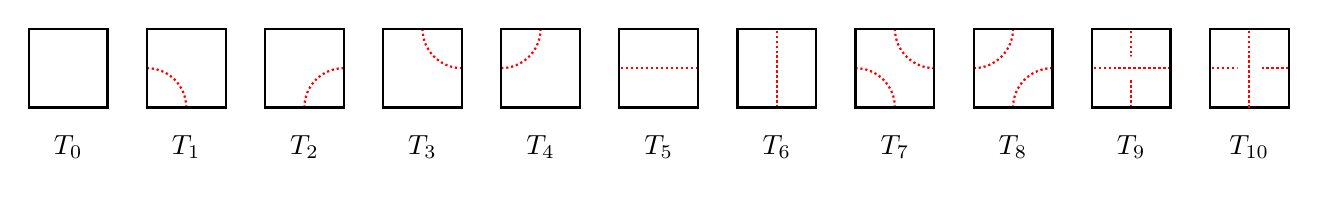
\begin{tikzpicture}
        \cell{0}{0}{1}{1}
        \( \lablnode{0.5}{-0.5}{$T_0$} \) 
        \cellA{1.5}{0}{2.5}{1}
        \( \lablnode{2}{-0.5}{$T_1$} \) 
        \cellB{3}{0}{4}{1}
        \( \lablnode{3.5}{-0.5}{$T_2$} \) 
        \cellC{4.5}{0}{5.5}{1}
        \( \lablnode{5}{-0.5}{$T_3$} \) 
        \cellD{6}{0}{7}{1}
        \( \lablnode{6.5}{-0.5}{$T_4$} \) 
        \cellE{7.5}{0}{8.5}{1}
        \( \lablnode{8}{-0.5}{$T_5$} \) 
        \cellF{9}{0}{10}{1}
        \( \lablnode{9.5}{-0.5}{$T_6$} \) 
        \cellG{10.5}{0}{11.5}{1}
        \( \lablnode{11}{-0.5}{$T_7$} \) 
        \cellH{12}{0}{13}{1}
        \( \lablnode{12.5}{-0.5}{$T_8$} \) 
        \cellI{13.5}{0}{14.5}{1}
        \( \lablnode{14}{-0.5}{$T_{9}$} \) 
        \cellJ{15}{0}{16}{1}
        \( \lablnode{15.5}{-0.5}{$T_{10}$} \) 
    \end{tikzpicture}
\end{center}

We denote the set of tiles $\mathbb{T}=\{T_0, \dots, T_{10}\}$. A \textit{mosaic} of size $(m,n)$ is an $m \times n$ matrix made up of elements from $\mathbb{T}$. Figure \ref{fig:example mosaic} shows an example mosaic of size $(5,7)$. We denote the set of all mosaics of size $(m,n)$ as $\mathbb{M}^{(m,n)}$. As there are $11$ elements in $\mathbb{T}$, there are $11^{mn}$ mosaics in $\mathbb{M}^{(m,n)}$. A \textit{mosaic system} is then a subset of $\mathbb{M}^{(m,n)}$ with some property. 

\begin{figure}[h!]
    \begin{center}
    \begin{subfigure}{0.4\textwidth}
        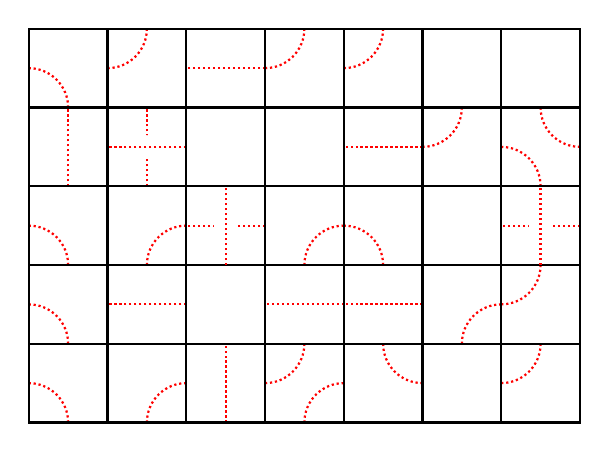
\begin{tikzpicture}
        % row1
        \cellA{0}{0}{1}{1}
        \cellB{1}{0}{2}{1}
        \cellF{2}{0}{3}{1}
        \cellH{3}{0}{4}{1}
        \cellC{4}{0}{5}{1}
        \cell{5}{0}{6}{1}
        \cellD{6}{0}{7}{1}
        % row2
        \cellA{0}{1}{1}{2}
        \cellE{1}{1}{2}{2}
        \cell{2}{1}{3}{2}
        \cellE{3}{1}{4}{2}
        \cellE{4}{1}{5}{2}
        \cellB{5}{1}{6}{2}
        \cellD{6}{1}{7}{2}
        % row3
        \cellA{0}{2}{1}{3}
        \cellB{1}{2}{2}{3}
        \cellJ{2}{2}{3}{3}
        \cellB{3}{2}{4}{3}
        \cellA{4}{2}{5}{3}
        \cell{5}{2}{6}{3}
        \cellJ{6}{2}{7}{3}
        % row4
        \cellF{0}{3}{1}{4}
        \cellI{1}{3}{2}{4}
        \cell{2}{3}{3}{4}
        \cell{3}{3}{4}{4}
        \cellE{4}{3}{5}{4}
        \cellD{5}{3}{6}{4}
        \cellG{6}{3}{7}{4}
        % row5
        \cellA{0}{4}{1}{5}
        \cellD{1}{4}{2}{5}
        \cellE{2}{4}{3}{5}
        \cellD{3}{4}{4}{5}
        \cellD{4}{4}{5}{5}
        \cell{5}{4}{6}{5}
        \cell{6}{4}{7}{5}
        \end{tikzpicture}
    \caption{A mosaic}
    \label{fig:example mosaic}
    \end{subfigure}
% \hfill
\hspace{0.05\textwidth}
\begin{subfigure}{0.4\textwidth}
    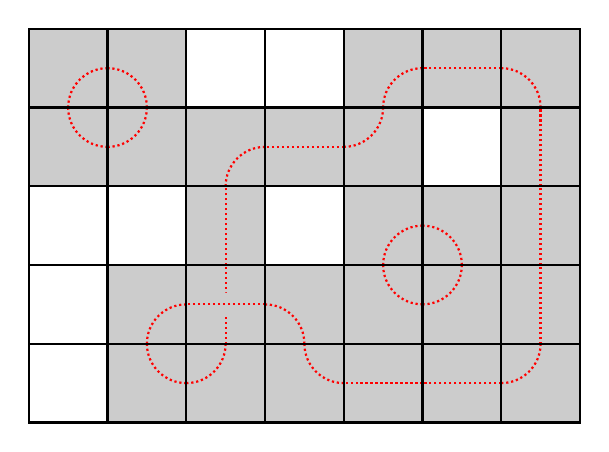
\begin{tikzpicture}
        % row1
        \cell{0}{0}{1}{1}
        \cellCf{1}{0}{2}{1}
        \cellDf{2}{0}{3}{1}
        \cellCf{3}{0}{4}{1}
        \cellEf{4}{0}{5}{1}
        \cellEf{5}{0}{6}{1}
        \cellDf{6}{0}{7}{1}
        % row2
        \cell{0}{1}{1}{2}
        \cellBf{1}{1}{2}{2}
        \cellIf{2}{1}{3}{2}
        \cellAf{3}{1}{4}{2}
        \cellCf{4}{1}{5}{2}
        \cellDf{5}{1}{6}{2}
        \cellFf{6}{1}{7}{2}
        % row3
        \cell{0}{2}{1}{3}
        \cell{1}{2}{2}{3}
        \cellFf{2}{2}{3}{3}
        \cell{3}{2}{4}{3}
        \cellBf{4}{2}{5}{3}
        \cellAf{5}{2}{6}{3}
        \cellFf{6}{2}{7}{3}
        % row4
        \cellCf{0}{3}{1}{4}
        \cellDf{1}{3}{2}{4}
        \cellBf{2}{3}{3}{4}
        \cellEf{3}{3}{4}{4}
        \cellDf{4}{3}{5}{4}
        \cell{5}{3}{6}{4}
        \cellFf{6}{3}{7}{4}
        % row5
        \cellBf{0}{4}{1}{5}
        \cellAf{1}{4}{2}{5}
        \cell{2}{4}{3}{5}
        \cell{3}{4}{4}{5}
        \cellBf{4}{4}{5}{5}
        \cellEf{5}{4}{6}{5}
        \cellAf{6}{4}{7}{5}
    \end{tikzpicture}
    \caption{A knot mosaic}
    \label{fig:example knot mosaic}
\end{subfigure}

\end{center}
\caption{Examples of mosaics of size $(5,7)$ made of tiles in $\mathbb{T}$}
\label{fig:example mosaics}
\end{figure}

We are interested in mosaics with the property of being \textit{suitably connected}, which is defined as follows. Consider an edge shared between two tiles in Figure \ref{fig:example mosaic}. The edge has either $0$, $1$, or $2$ dotted lines drawn from its midpoint. Also note that the edges of the tiles on the boundary of the matrix are not shared by another tile. Therefore these edges only have $0$ or $1$ dotted lines drawn from their midpoint. A mosaic is suitably connected if all edges have $0$ or $2$ dotted lines drawn from their midpoint.

Lomonaco and Kauffman \cite{Lomonaco08} call these \textit{knot mosaics} because, other than the mosaic consisting of all $T_0$ tiles, the dotted lines form  \textit{knots}. Following the notation in \cite{Oh2014} we denote the subset of mosaics of size $(m,n)$ that are knot mosaics as $\mathbb{K}^{(m,n)}$. Figure \ref{fig:example knot mosaic} shows a knot mosaic of size $(5,7)$ that contains $3$ knots, with the tiles that make up the knots highlighted in gray. Note that a mosaic can contain knots isomorphic to the unknot, as well as knots that encompass other knots. 

Let $k_{m,n} = |\mathbb{K}^{(m,n)}|$ be the number of knot mosaics of size $(m,n)$. First notice that if either $m$ or $n$ is $1$, one can only construct a knot mosaic using $T_0$ tiles, so $k_{m,1} = k_{1,n} = 1.$ Oh et al. \cite{Oh2014} showed the following for $m,n \geq 2$.

\begin{thm}[\cite{Oh2014}]
    \label{thm:Oh2014}
    The number of knot mosaics of size $(m,n)$ for $m,n \geq 2$ is $k_{m,n} = 2 \left\| (X_{m-2}+O_{m-2})^{n-2} \right\|$, where $X_{m-2}$ and $O_{m-2}$ are $2^{m-2} \times 2^{m-2}$ matrices defined as

    $$ X_{k+1} = \begin{bmatrix}
        X_k & O_k \\
        O_k & X_k
    \end{bmatrix}
    \text{ and }
    O_{k+1} = \begin{bmatrix}
        O_k & X_k \\
        X_k & 4O_k
    \end{bmatrix}, $$
    
    for $k=0,1,\dots,m-3$, and $X_0 = O_0 = \begin{bmatrix} 1 \\ \end{bmatrix}$. Here $\left\| N \right\|$ denotes the sum of elements of matrix $N$.
\end{thm}

Oh and colleagues refer to these matrices $X_k$ and $O_k$ as \textit{state matrices}. The authors utilize this state matrix recursion to bound the growth rate of knot mosaics $\delta = \lim_{n \to \infty} k_{n,n}^{\frac{1}{n^2}}$ \cite{Oh2016, Oh2019, Choi2024}, and Oh further adapts the method to solve problems in monomer and dimer tilings \cite{Oh2018Aztec, Oh2019tiling}. An unexamined direction in this research program is modifying the suitably connected property. This motivates us to introduce \textit{messy knot mosaics}.


\section{Messy Knot Mosaics}\label{section:messy mosaics}

\begin{definition}
    A \textit{messy knot mosaic} is a mosaic that contains at least one knot. 
\end{definition}

Figure \ref{fig:messy mosaic example} shows two examples of messy knot mosaic of size $(5,7)$ that contains $3$ knots\footnote{Certain permutations of $\{T_1, T_2, T_3, T_4\}$ and $\{T_7,T_8\}$ can make shapes that appear to be knots but have hanging connections, as seen in the $(0,4)$ position in the right example in Figure \ref{fig:messy mosaic example}. These are not considered knots by this paper and all referenced works.}, with the tiles that make up the knots highlighted in gray. All knot mosaics are messy knot mosaics.

\begin{figure}[h!]
    \begin{center}

\begin{subfigure}{0.4\textwidth}
    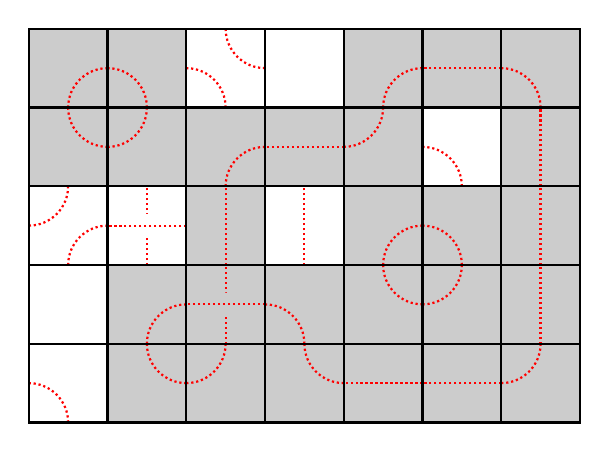
\begin{tikzpicture}
       % row1
        \cellA{0}{0}{1}{1}
        \cellCf{1}{0}{2}{1}
        \cellDf{2}{0}{3}{1}
        \cellCf{3}{0}{4}{1}
        \cellEf{4}{0}{5}{1}
        \cellEf{5}{0}{6}{1}
        \cellDf{6}{0}{7}{1}
        % row2
        \cell{0}{1}{1}{2}
        \cellBf{1}{1}{2}{2}
        \cellIf{2}{1}{3}{2}
        \cellAf{3}{1}{4}{2}
        \cellCf{4}{1}{5}{2}
        \cellDf{5}{1}{6}{2}
        \cellFf{6}{1}{7}{2}
        % row3
        \cellH{0}{2}{1}{3}
        \cellI{1}{2}{2}{3}
        \cellFf{2}{2}{3}{3}
        \cellF{3}{2}{4}{3}
        \cellBf{4}{2}{5}{3}
        \cellAf{5}{2}{6}{3}
        \cellFf{6}{2}{7}{3}
        % row4
        \cellCf{0}{3}{1}{4}
        \cellDf{1}{3}{2}{4}
        \cellBf{2}{3}{3}{4}
        \cellEf{3}{3}{4}{4}
        \cellDf{4}{3}{5}{4}
        \cellA{5}{3}{6}{4}
        \cellFf{6}{3}{7}{4}
        % row5
        \cellBf{0}{4}{1}{5}
        \cellAf{1}{4}{2}{5}
        \cellG{2}{4}{3}{5}
        \cell{3}{4}{4}{5}
        \cellBf{4}{4}{5}{5}
        \cellEf{5}{4}{6}{5}
        \cellAf{6}{4}{7}{5}
    \end{tikzpicture}
\end{subfigure}
% \hfill
\hspace{0.05\textwidth}
\begin{subfigure}{0.4\textwidth}
        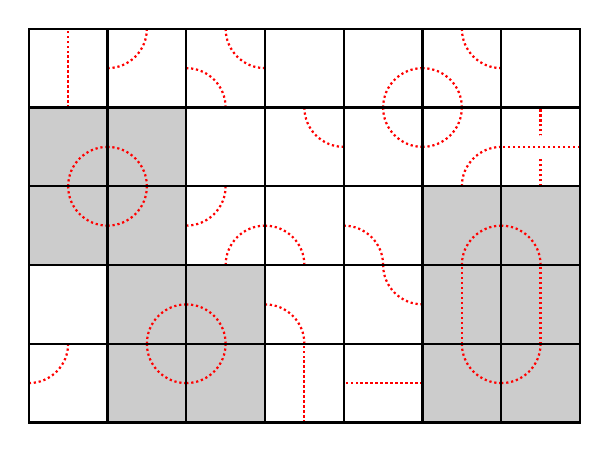
\begin{tikzpicture}
        % row1
        \cellD{0}{0}{1}{1}
        \cellCf{1}{0}{2}{1}
        \cellDf{2}{0}{3}{1}
        \cellF{3}{0}{4}{1}
        \cellE{4}{0}{5}{1}
        \cellCf{5}{0}{6}{1}
        \cellDf{6}{0}{7}{1}
        % row2
        \cell{0}{1}{1}{2}
        \cellBf{1}{1}{2}{2}
        \cellAf{2}{1}{3}{2}
        \cellA{3}{1}{4}{2}
        \cellC{4}{1}{5}{2}
        \cellFf{5}{1}{6}{2}
        \cellFf{6}{1}{7}{2}
        % row3
        \cellCf{0}{2}{1}{3}
        \cellDf{1}{2}{2}{3}
        \cellH{2}{2}{3}{3}
        \cellA{3}{2}{4}{3}
        \cellA{4}{2}{5}{3}
        \cellBf{5}{2}{6}{3}
        \cellAf{6}{2}{7}{3}
        % row4
        \cellBf{0}{3}{1}{4}
        \cellAf{1}{3}{2}{4}
        \cell{2}{3}{3}{4}
        \cellC{3}{3}{4}{4}
        \cellC{4}{3}{5}{4}
        \cellH{5}{3}{6}{4}
        \cellI{6}{3}{7}{4}
        % row5
        \cellF{0}{4}{1}{5}
        \cellD{1}{4}{2}{5}
        \cellG{2}{4}{3}{5}
        \cell{3}{4}{4}{5}
        \cellB{4}{4}{5}{5}
        \cellG{5}{4}{6}{5}
        \cell{6}{4}{7}{5}
    \end{tikzpicture}
\end{subfigure}

\end{center}
\caption{Messy knot mosaics}
\label{fig:messy mosaic example}
\end{figure}

It turns out to be simpler to enumerate the number of mosaics that \textit{do not} contain a knot. Therefore, let $\mathbb{S}^{(m,n)}$ be the set of mosaics that do not contain a knot, and let $|\mathbb{S}^{(m,n)}| = s_{m,n}$. Clearly the number of messy knot mosaics is then $11^{mn} - s_{m,n}$.

First, note that the knot made up of the least amount of cells is this: 

\begin{center}
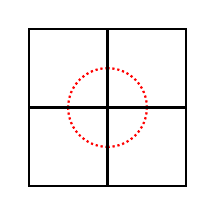
\begin{tikzpicture}
    % row1
    \cellC{0}{0}{1}{1}
    \cellD{1}{0}{2}{1}
    % row2
    \cellB{0}{1}{1}{2}
    \cellA{1}{1}{2}{2}
\end{tikzpicture}
\end{center}

We can then conclude that $s_{n,1}=11^n$, and $s_{2,2} = 11^4 - 1$. For $n,m \geq 2$, we first define the state matrices for messy knot mosaics.

\begin{definition}

Define $A(2) = \begin{bmatrix}
11^2 & 1 \\
-1 & 1
\end{bmatrix}$. We recursively define $A(k+1) \in \mathbb{N}^{2^{k} \times 2^{k}}$ given $A(k)$. Begin by writing
$
A(k) = \begin{bmatrix}
A_{0,0} & A_{0,1} \\
A_{1,0} & A_{1,1}
\end{bmatrix}
$, where the block matrices $A_{i,j}$ are square block matrices of size $2^{k-1} \times 2^{k-1}$. We then have

$$
A(k+1) = \begin{bmatrix}
    11A_{0,0} & \frac{1}{11}A_{0,0} & 11A_{0,1} & A_{0,1} \\
    -\frac{1}{11}A_{0,0} & \frac{1}{11}A_{0,0} & 4A_{0,1} & A_{0,1} \\
    11A_{1,0} & -4A_{1,0} & 11A_{1,1}  & A_{1,1} \\
    A_{1,0} & -A_{1,0} & A_{1,1} & 11A_{1,1} \\
\end{bmatrix}.
$$

Construct $A(m)$ by starting with $k=2$ and recursing until $k=m$. 

\end{definition}

\begin{thm}
\label{thm: messy mosaics}
The number of mosaics of size $(m,n)$ that \textit{do not} contain a knot is the $(0,0)$ entry of $A(m)^n$.
\end{thm}

\section{Preliminaries}

We begin by defining a mapping $f$ between $\mathbb{M}^{(m,n)}$ to a \textit{binary lattice} of size $(m,n)$. A binary lattice of size $(m,n)$ is a rectangular lattice of $m+1$ by $n+1$ vertices, in which the boundary vertices are labeled $0$, and the interior vertices are either $0$ or $1$. An example of a binary lattice of size $(5,7)$ is shown on the right of Figure \ref{fig:example of f mapping}. Also let $\mathbb{L}^{(m,n)}$ be the set of all binary lattices of size $(m,n)$, which gives $\left|\mathbb{L}^{(m,n)}\right| = 2^{(m-1)(n-1)}$. 

\begin{definition}

$f: \mathbb{M}^{(m,n)} \to \mathbb{L}^{(m,n)}$ takes a mosaic and labels each vertex with the following rule. If the vertex is surrounded by an even number of knots (including $0$ knots), label it $0$. If the vertex is surrounded by an odd number of knots, label it $1$. Removing the red dotted lines from the tiles gives the binary lattice. 
    
\end{definition}

Similarly, define the \textit{preimage} of a set $L$ under $f$ to be

$$f^{-1}(L) = \{m \in \mathbb{M}^{(m,n)} | f(m) \in L\}.$$

We want to compute $s_{m,n}$ by computing $f^{-1}(\ell)$ for each $\ell \in \mathbb{L}^{(m,n)}$, and then summing over all $\ell$. We begin by finding a simple way to compute $f^{-1}(\ell)$ for a binary lattice $\ell$ by examining the structure of $\ell$.

\begin{figure}
\begin{center}
    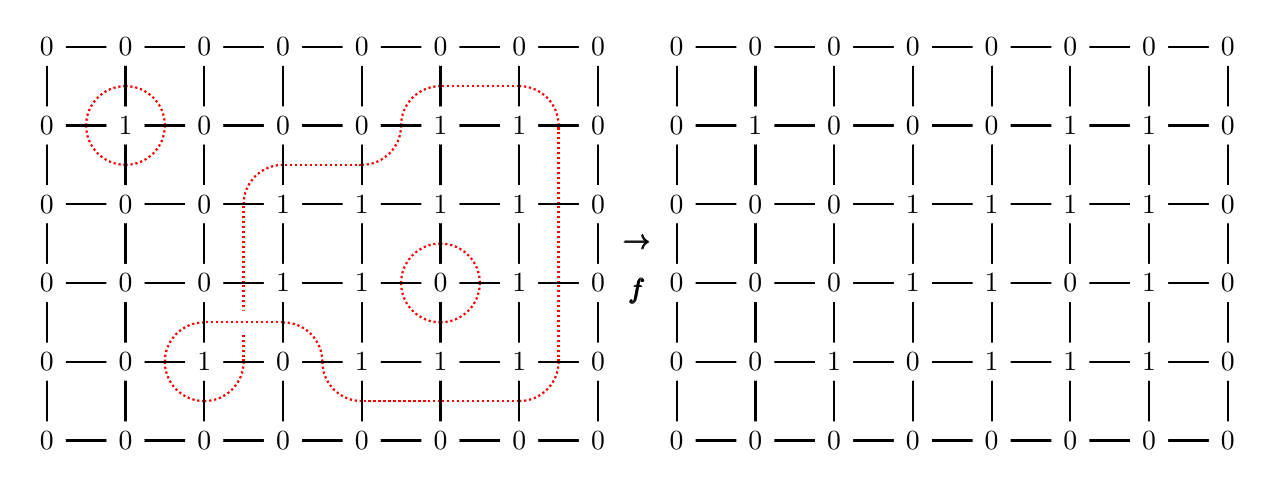
\begin{tikzpicture}
        % row1
        \cell{0}{0}{1}{1}
        \cellC{1}{0}{2}{1}
        \cellD{2}{0}{3}{1}
        \cellC{3}{0}{4}{1}
        \cellE{4}{0}{5}{1}
        \cellE{5}{0}{6}{1}
        \cellD{6}{0}{7}{1}
        % row2
        \cell{0}{1}{1}{2}
        \cellB{1}{1}{2}{2}
        \cellI{2}{1}{3}{2}
        \cellA{3}{1}{4}{2}
        \cellC{4}{1}{5}{2}
        \cellD{5}{1}{6}{2}
        \cellF{6}{1}{7}{2}
        % row3
        \cell{0}{2}{1}{3}
        \cell{1}{2}{2}{3}
        \cellF{2}{2}{3}{3}
        \cell{3}{2}{4}{3}
        \cellB{4}{2}{5}{3}
        \cellA{5}{2}{6}{3}
        \cellF{6}{2}{7}{3}
        % row4
        \cellC{0}{3}{1}{4}
        \cellD{1}{3}{2}{4}
        \cellB{2}{3}{3}{4}
        \cellE{3}{3}{4}{4}
        \cellD{4}{3}{5}{4}
        \cell{5}{3}{6}{4}
        \cellF{6}{3}{7}{4}
        % row5
        \cellB{0}{4}{1}{5}
        \cellA{1}{4}{2}{5}
        \cell{2}{4}{3}{5}
        \cell{3}{4}{4}{5}
        \cellB{4}{4}{5}{5}
        \cellE{5}{4}{6}{5}
        \cellA{6}{4}{7}{5}
        % label for row1
        \( \lablvertex{0}{0}{$0$} \)
        \( \lablvertex{1}{0}{$0$} \)
        \( \lablvertex{2}{0}{$0$} \)
        \( \lablvertex{3}{0}{$0$} \)
        \( \lablvertex{4}{0}{$0$} \)
        \( \lablvertex{5}{0}{$0$} \)
        \( \lablvertex{6}{0}{$0$} \)
        \( \lablvertex{7}{0}{$0$} \)
        % label for row1
        \( \lablvertex{0}{1}{$0$} \)
        \( \lablvertex{1}{1}{$0$} \)
        \( \lablvertex{2}{1}{$1$} \)
        \( \lablvertex{3}{1}{$0$} \)
        \( \lablvertex{4}{1}{$1$} \)
        \( \lablvertex{5}{1}{$1$} \)
        \( \lablvertex{6}{1}{$1$} \)
        \( \lablvertex{7}{1}{$0$} \)
        % label for row1
        \( \lablvertex{0}{2}{$0$} \)
        \( \lablvertex{1}{2}{$0$} \)
        \( \lablvertex{2}{2}{$0$} \)
        \( \lablvertex{3}{2}{$1$} \)
        \( \lablvertex{4}{2}{$1$} \)
        \( \lablvertex{5}{2}{$0$} \)
        \( \lablvertex{6}{2}{$1$} \)
        \( \lablvertex{7}{2}{$0$} \)
        % label for row1
        \( \lablvertex{0}{3}{$0$} \)
        \( \lablvertex{1}{3}{$0$} \)
        \( \lablvertex{2}{3}{$0$} \)
        \( \lablvertex{3}{3}{$1$} \)
        \( \lablvertex{4}{3}{$1$} \)
        \( \lablvertex{5}{3}{$1$} \)
        \( \lablvertex{6}{3}{$1$} \)
        \( \lablvertex{7}{3}{$0$} \)
        % label for row1
        \( \lablvertex{0}{4}{$0$} \)
        \( \lablvertex{1}{4}{$1$} \)
        \( \lablvertex{2}{4}{$0$} \)
        \( \lablvertex{3}{4}{$0$} \)
        \( \lablvertex{4}{4}{$0$} \)
        \( \lablvertex{5}{4}{$1$} \)
        \( \lablvertex{6}{4}{$1$} \)
        \( \lablvertex{7}{4}{$0$} \)
        % label for row1
        \( \lablvertex{0}{5}{$0$} \)
        \( \lablvertex{1}{5}{$0$} \)
        \( \lablvertex{2}{5}{$0$} \)
        \( \lablvertex{3}{5}{$0$} \)
        \( \lablvertex{4}{5}{$0$} \)
        \( \lablvertex{5}{5}{$0$} \)
        \( \lablvertex{6}{5}{$0$} \)
        \( \lablvertex{7}{5}{$0$} \)
        % arrow
        \( \lablnode{7.5}{2.5}{$\pmb{\to}$} \)
        % 
        \( \lablnode{7.5}{1.9}{$\pmb{f}$} \)

        % row1
        \cell{8}{0}{9}{1}
        \cell{9}{0}{10}{1}
        \cell{10}{0}{11}{1}
        \cell{11}{0}{12}{1}
        \cell{12}{0}{13}{1}
        \cell{13}{0}{14}{1}
        \cell{14}{0}{15}{1}
        % row2
        \cell{8}{1}{9}{2}
        \cell{9}{1}{10}{2}
        \cell{10}{1}{11}{2}
        \cell{11}{1}{12}{2}
        \cell{12}{1}{13}{2}
        \cell{13}{1}{14}{2}
        \cell{14}{1}{15}{2}
        % row3
        \cell{8}{2}{9}{3}
        \cell{9}{2}{10}{3}
        \cell{10}{2}{11}{3}
        \cell{11}{2}{12}{3}
        \cell{12}{2}{13}{3}
        \cell{13}{2}{14}{3}
        \cell{14}{2}{15}{3}
        % row4
        \cell{8}{3}{9}{4}
        \cell{9}{3}{10}{4}
        \cell{10}{3}{11}{4}
        \cell{11}{3}{12}{4}
        \cell{12}{3}{13}{4}
        \cell{13}{3}{14}{4}
        \cell{14}{3}{15}{4}
        % row5
        \cell{8}{4}{9}{5}
        \cell{9}{4}{10}{5}
        \cell{10}{4}{11}{5}
        \cell{11}{4}{12}{5}
        \cell{12}{4}{13}{5}
        \cell{13}{4}{14}{5}
        \cell{14}{4}{15}{5}

        % label for row1
        \( \lablvertex{8}{0}{$0$} \)
        \( \lablvertex{9}{0}{$0$} \)
        \( \lablvertex{10}{0}{$0$} \)
        \( \lablvertex{11}{0}{$0$} \)
        \( \lablvertex{12}{0}{$0$} \)
        \( \lablvertex{13}{0}{$0$} \)
        \( \lablvertex{14}{0}{$0$} \)
        \( \lablvertex{15}{0}{$0$} \)
        % label for row1
        \( \lablvertex{8}{1}{$0$} \)
        \( \lablvertex{9}{1}{$0$} \)
        \( \lablvertex{10}{1}{$1$} \)
        \( \lablvertex{11}{1}{$0$} \)
        \( \lablvertex{12}{1}{$1$} \)
        \( \lablvertex{13}{1}{$1$} \)
        \( \lablvertex{14}{1}{$1$} \)
        \( \lablvertex{15}{1}{$0$} \)
        % label for row1
        \( \lablvertex{8}{2}{$0$} \)
        \( \lablvertex{9}{2}{$0$} \)
        \( \lablvertex{10}{2}{$0$} \)
        \( \lablvertex{11}{2}{$1$} \)
        \( \lablvertex{12}{2}{$1$} \)
        \( \lablvertex{13}{2}{$0$} \)
        \( \lablvertex{14}{2}{$1$} \)
        \( \lablvertex{15}{2}{$0$} \)
        % label for row1
        \( \lablvertex{8}{3}{$0$} \)
        \( \lablvertex{9}{3}{$0$} \)
        \( \lablvertex{10}{3}{$0$} \)
        \( \lablvertex{11}{3}{$1$} \)
        \( \lablvertex{12}{3}{$1$} \)
        \( \lablvertex{13}{3}{$1$} \)
        \( \lablvertex{14}{3}{$1$} \)
        \( \lablvertex{15}{3}{$0$} \)
        % label for row1
        \( \lablvertex{8}{4}{$0$} \)
        \( \lablvertex{9}{4}{$1$} \)
        \( \lablvertex{10}{4}{$0$} \)
        \( \lablvertex{11}{4}{$0$} \)
        \( \lablvertex{12}{4}{$0$} \)
        \( \lablvertex{13}{4}{$1$} \)
        \( \lablvertex{14}{4}{$1$} \)
        \( \lablvertex{15}{4}{$0$} \)
        % label for row1
        \( \lablvertex{8}{5}{$0$} \)
        \( \lablvertex{9}{5}{$0$} \)
        \( \lablvertex{10}{5}{$0$} \)
        \( \lablvertex{11}{5}{$0$} \)
        \( \lablvertex{12}{5}{$0$} \)
        \( \lablvertex{13}{5}{$0$} \)
        \( \lablvertex{14}{5}{$0$} \)
        \( \lablvertex{15}{5}{$0$} \)

    \end{tikzpicture}
\end{center}
\caption{$f$ applied to the left mosaic in Figure \ref{fig:messy mosaic example}, resulting in a binary lattice}
\label{fig:example of f mapping}
\end{figure}

\begin{definition}
    Let a \textit{cell} be the portion of the binary lattice that an individual tile maps to, and let $C$ be the set of unique cells. 
\end{definition}

For convenience, we give a pair of indexes to each of the $|C| = 2^4$ unique cells. The first index is the binary number formed by reading the bottom two vertices from left to right. The second index is the binary number formed by reading the top two vertices from left to right. Below is a diagram of all $2^4$ cells with their indexes listed below.

\begin{center}
    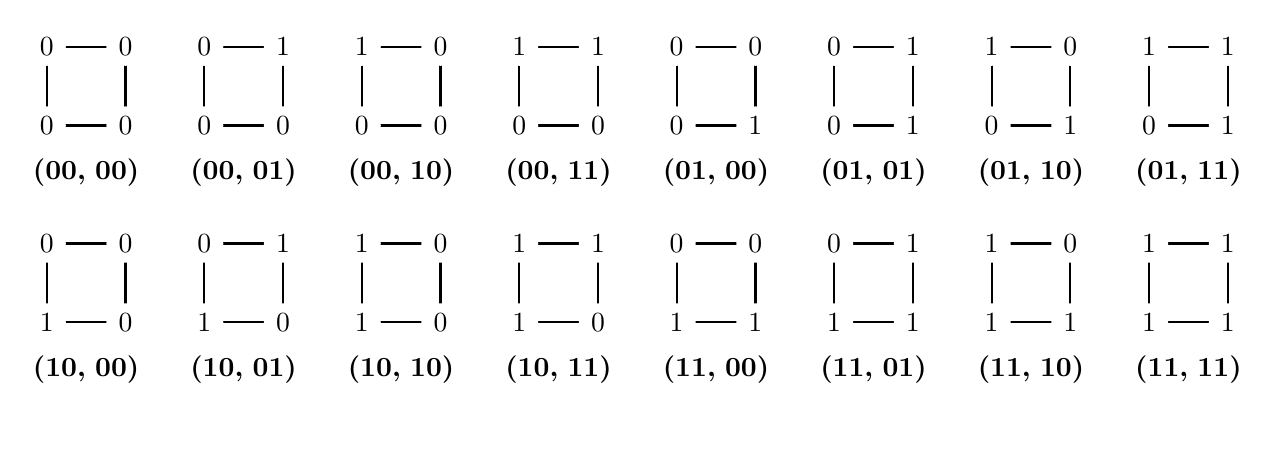
\begin{tikzpicture}
        % row1
        \cell{0}{-0.5}{1}{0.5}
        \cell{2}{-0.5}{3}{0.5}
        \cell{4}{-0.5}{5}{0.5}
        \cell{6}{-0.5}{7}{0.5}
        \cell{8}{-0.5}{9}{0.5}
        \cell{10}{-0.5}{11}{0.5}
        \cell{12}{-0.5}{13}{0.5}
        \cell{14}{-0.5}{15}{0.5}
        % row2
        \cell{0}{2}{1}{3}
        \cell{2}{2}{3}{3}
        \cell{4}{2}{5}{3}
        \cell{6}{2}{7}{3}
        \cell{8}{2}{9}{3}
        \cell{10}{2}{11}{3}
        \cell{12}{2}{13}{3}
        \cell{14}{2}{15}{3}

        % label for row 1
        \( \lablvertex{0}{-0.5}{$1$} \)
        \( \lablvertex{1}{-0.5}{$0$} \)
        \( \lablvertex{2}{-0.5}{$1$} \)
        \( \lablvertex{3}{-0.5}{$0$} \)
        \( \lablvertex{4}{-0.5}{$1$} \)
        \( \lablvertex{5}{-0.5}{$0$} \)
        \( \lablvertex{6}{-0.5}{$1$} \)
        \( \lablvertex{7}{-0.5}{$0$} \)
        \( \lablvertex{8}{-0.5}{$1$} \)
        \( \lablvertex{9}{-0.5}{$1$} \)
        \( \lablvertex{10}{-0.5}{$1$} \)
        \( \lablvertex{11}{-0.5}{$1$} \)
        \( \lablvertex{12}{-0.5}{$1$} \)
        \( \lablvertex{13}{-0.5}{$1$} \)
        \( \lablvertex{14}{-0.5}{$1$} \)
        \( \lablvertex{15}{-0.5}{$1$} \)
        
        % label for row 2
        \( \lablvertex{0}{0.5}{$0$} \)
        \( \lablvertex{1}{0.5}{$0$} \)
        \( \lablvertex{2}{0.5}{$0$} \)
        \( \lablvertex{3}{0.5}{$1$} \)
        \( \lablvertex{4}{0.5}{$1$} \)
        \( \lablvertex{5}{0.5}{$0$} \)
        \( \lablvertex{6}{0.5}{$1$} \)
        \( \lablvertex{7}{0.5}{$1$} \)
        \( \lablvertex{8}{0.5}{$0$} \)
        \( \lablvertex{9}{0.5}{$0$} \)
        \( \lablvertex{10}{0.5}{$0$} \)
        \( \lablvertex{11}{0.5}{$1$} \)
        \( \lablvertex{12}{0.5}{$1$} \)
        \( \lablvertex{13}{0.5}{$0$} \)
        \( \lablvertex{14}{0.5}{$1$} \)
        \( \lablvertex{15}{0.5}{$1$} \)

        % label for row 3
        \( \lablvertex{0}{2}{$0$} \)
        \( \lablvertex{1}{2}{$0$} \)
        \( \lablvertex{2}{2}{$0$} \)
        \( \lablvertex{3}{2}{$0$} \)
        \( \lablvertex{4}{2}{$0$} \)
        \( \lablvertex{5}{2}{$0$} \)
        \( \lablvertex{6}{2}{$0$} \)
        \( \lablvertex{7}{2}{$0$} \)
        \( \lablvertex{8}{2}{$0$} \)
        \( \lablvertex{9}{2}{$1$} \)
        \( \lablvertex{10}{2}{$0$} \)
        \( \lablvertex{11}{2}{$1$} \)
        \( \lablvertex{12}{2}{$0$} \)
        \( \lablvertex{13}{2}{$1$} \)
        \( \lablvertex{14}{2}{$0$} \)
        \( \lablvertex{15}{2}{$1$} \)
        
        % label for row 4
        \( \lablvertex{0}{3}{$0$} \)
        \( \lablvertex{1}{3}{$0$} \)
        \( \lablvertex{2}{3}{$0$} \)
        \( \lablvertex{3}{3}{$1$} \)
        \( \lablvertex{4}{3}{$1$} \)
        \( \lablvertex{5}{3}{$0$} \)
        \( \lablvertex{6}{3}{$1$} \)
        \( \lablvertex{7}{3}{$1$} \)
        \( \lablvertex{8}{3}{$0$} \)
        \( \lablvertex{9}{3}{$0$} \)
        \( \lablvertex{10}{3}{$0$} \)
        \( \lablvertex{11}{3}{$1$} \)
        \( \lablvertex{12}{3}{$1$} \)
        \( \lablvertex{13}{3}{$0$} \)
        \( \lablvertex{14}{3}{$1$} \)
        \( \lablvertex{15}{3}{$1$} \)

        % numbers row 1
        \( \lablnode{0.5}{1.4}{\textbf{(}$\mathbf{00}$\textbf{,} $\mathbf{00}$\textbf{)}} \)
        \( \lablnode{2.5}{1.4}{\textbf{(}$\mathbf{00}$\textbf{,} $\mathbf{01}$\textbf{)}} \)
        \( \lablnode{4.5}{1.4}{\textbf{(}$\mathbf{00}$\textbf{,} $\mathbf{10}$\textbf{)}} \)
        \( \lablnode{6.5}{1.4}{\textbf{(}$\mathbf{00}$\textbf{,} $\mathbf{11}$\textbf{)}} \)
        \( \lablnode{8.5}{1.4}{\textbf{(}$\mathbf{01}$\textbf{,} $\mathbf{00}$\textbf{)}} \)
        \( \lablnode{10.5}{1.4}{\textbf{(}$\mathbf{01}$\textbf{,} $\mathbf{01}$\textbf{)}} \)
        \( \lablnode{12.5}{1.4}{\textbf{(}$\mathbf{01}$\textbf{,} $\mathbf{10}$\textbf{)}} \)
        \( \lablnode{14.5}{1.4}{\textbf{(}$\mathbf{01}$\textbf{,} $\mathbf{11}$\textbf{)}} \)
        
        % numbers row 2
        \( \lablnode{0.5}{-1.1}{\textbf{(}$\mathbf{10}$\textbf{,} $\mathbf{00}$\textbf{)}} \)
        \( \lablnode{2.5}{-1.1}{\textbf{(}$\mathbf{10}$\textbf{,} $\mathbf{01}$\textbf{)}} \)
        \( \lablnode{4.5}{-1.1}{\textbf{(}$\mathbf{10}$\textbf{,} $\mathbf{10}$\textbf{)}} \)
        \( \lablnode{6.5}{-1.1}{\textbf{(}$\mathbf{10}$\textbf{,} $\mathbf{11}$\textbf{)}} \)
        \( \lablnode{8.5}{-1.1}{\textbf{(}$\mathbf{11}$\textbf{,} $\mathbf{00}$\textbf{)}} \)
        \( \lablnode{10.5}{-1.1}{\textbf{(}$\mathbf{11}$\textbf{,} $\mathbf{01}$\textbf{)}} \)
        \( \lablnode{12.5}{-1.1}{\textbf{(}$\mathbf{11}$\textbf{,} $\mathbf{10}$\textbf{)}} \)
        \( \lablnode{14.5}{-1.1}{\textbf{(}$\mathbf{11}$\textbf{,} $\mathbf{11}$\textbf{)}} \)
    \end{tikzpicture}
\end{center}

Next let $u_{(i,j)}$ be the number of tiles in $\mathbb{T}$ that can map to cell $(i,j)$. These values are simple to calculate, as each tile in $\mathbb{T}$ can only be part of a knot in certain ways. For example, $u_{(00, 01)} = 1$, as cell $(00,01)$ can only be formed by a mosaic with $T_3$ in that location. We can see that $u_{(01,10)}=4$, as cell $(01,10)$ can be from the $T_7,T_8,T_9$, or $T_{10}$ tiles. Finally, we have $u_{(00,00)}=11$, as any tile can fail to contribute to forming a knot. Table \ref{tbl:Preimage of binary cell lattice} summarizes the tiles in the preimage for each cell $(i,j)$. 

\begin{table}[h!]
    \begin{center}
        \begin{tabular}{ |c|l|c|c|l|c| } 
            \hline
            \textbf{Cell (}$\mathbf{i}$\textbf{,} $\mathbf{j}$\textbf{)} & \textbf{Preimage} & $\mathbf{u_{(i,j)}}$ & \textbf{Cell (}$\mathbf{i}$\textbf{,} $\mathbf{j}$\textbf{)} & \textbf{Preimage} & $\mathbf{u_{(i,j)}}$ \\ 
            \hline
            $(00, 00)$ & $\mathbb{T}$ & $11$ & $(10, 00)$ & $T_1$ & $1$ \\
            \hline
            $(00, 01)$ & $T_3$ & $1$ & $(10, 01)$ & $T_{7},T_{8},T_{9},T_{10}$ & $4$ \\
            \hline
            $(00, 10)$ & $T_4$ & $1$ & $(10, 10)$ & $T_6$ & $1$ \\
            \hline
            $(00, 11)$ & $T_5$ & $1$ & $(10, 11)$ & $T_2$ & $1$ \\
            \hline
            $(01, 00)$ & $T_2$ & $1$ & $(11, 00)$ & $T_5$ & $1$ \\
            \hline
            $(01, 01)$ & $T_6$ & $1$ & $(11, 01)$ & $T_4$ & $1$ \\
            \hline
            $(01, 10)$ & $T_{7},T_{8},T_{9},T_{10}$ & $4$ & $(11, 10)$ & $T_1$ & $1$ \\
            \hline
            $(01, 11)$ & $T_1$ & $1$ & $(11, 11)$ & $\mathbb{T}$ & $11$ \\
            \hline
        \end{tabular}
        \caption{Preimages of each unique cell}
        \label{tbl:Preimage of binary cell lattice}
    \end{center}
\end{table}

However, for some binary lattice $\ell$ the quantity 

\begin{equation}
    U(\ell) := \prod_{\text{Cell }(i,j) \in \ell} u_{(i,j)}
\end{equation}

is not necessarily equal to $\left|f^{-1}\left(\{\ell\}\right)\right|$, as $U(\ell)$ does not \textit{just} count the number of mosaics that map to $\ell$ under $f$. 

\begin{exmp}

Consider the following binary lattices for $s_{4,2}$. 

\begin{center}
    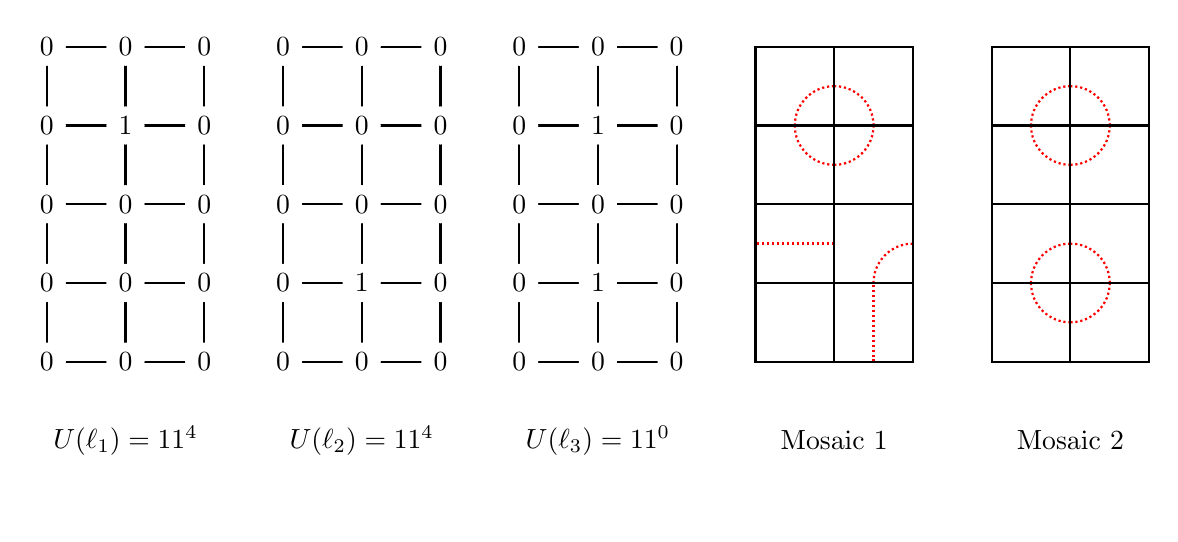
\begin{tikzpicture}

        % row1
        \cell{-3}{0}{-2}{1}
        \cell{-3}{1}{-2}{2}
        \cell{-3}{2}{-2}{3}
        \cell{-3}{3}{-2}{4}
        \cell{-2}{0}{-1}{1}
        \cell{-2}{1}{-1}{2}
        \cell{-2}{2}{-1}{3}
        \cell{-2}{3}{-1}{4}

        \( \lablnode{-2}{-1}{$U(\ell_{1}) = 11^4$} \)

        \( \lablvertex{-3}{0}{$0$} \)
        \( \lablvertex{-2}{0}{$0$} \)
        \( \lablvertex{-1}{0}{$0$} \)

        \( \lablvertex{-3}{1}{$0$} \)
        \( \lablvertex{-2}{1}{$0$} \)
        \( \lablvertex{-1}{1}{$0$} \)

        \( \lablvertex{-3}{2}{$0$} \)
        \( \lablvertex{-2}{2}{$0$} \)
        \( \lablvertex{-1}{2}{$0$} \)

        \( \lablvertex{-3}{3}{$0$} \)
        \( \lablvertex{-2}{3}{$1$} \)
        \( \lablvertex{-1}{3}{$0$} \)

        \( \lablvertex{-3}{4}{$0$} \)
        \( \lablvertex{-2}{4}{$0$} \)
        \( \lablvertex{-1}{4}{$0$} \)

        % row1
        \cell{0}{0}{1}{1}
        \cell{0}{1}{1}{2}
        \cell{0}{2}{1}{3}
        \cell{0}{3}{1}{4}
        \cell{1}{0}{2}{1}
        \cell{1}{1}{2}{2}
        \cell{1}{2}{2}{3}
        \cell{1}{3}{2}{4}

        \( \lablnode{1}{-1}{$U(\ell_{2}) =11^4$} \)
        
        \( \lablvertex{0}{0}{$0$} \)
        \( \lablvertex{1}{0}{$0$} \)
        \( \lablvertex{2}{0}{$0$} \)

        \( \lablvertex{0}{1}{$0$} \)
        \( \lablvertex{1}{1}{$1$} \)
        \( \lablvertex{2}{1}{$0$} \)

        \( \lablvertex{0}{2}{$0$} \)
        \( \lablvertex{1}{2}{$0$} \)
        \( \lablvertex{2}{2}{$0$} \)

        \( \lablvertex{0}{3}{$0$} \)
        \( \lablvertex{1}{3}{$0$} \)
        \( \lablvertex{2}{3}{$0$} \)

        \( \lablvertex{0}{4}{$0$} \)
        \( \lablvertex{1}{4}{$0$} \)
        \( \lablvertex{2}{4}{$0$} \)

        % row1
        \cell{3}{0}{4}{1}
        \cell{3}{1}{4}{2}
        \cell{3}{2}{4}{3}
        \cell{3}{3}{4}{4}
        \cell{4}{0}{5}{1}
        \cell{4}{1}{5}{2}
        \cell{4}{2}{5}{3}
        \cell{4}{3}{5}{4}

        \( \lablnode{4}{-1}{$U(\ell_{3}) = 11^0$} \)

        \( \lablvertex{3}{0}{$0$} \)
        \( \lablvertex{4}{0}{$0$} \)
        \( \lablvertex{5}{0}{$0$} \)

        \( \lablvertex{3}{1}{$0$} \)
        \( \lablvertex{4}{1}{$1$} \)
        \( \lablvertex{5}{1}{$0$} \)

        \( \lablvertex{3}{2}{$0$} \)
        \( \lablvertex{4}{2}{$0$} \)
        \( \lablvertex{5}{2}{$0$} \)

        \( \lablvertex{3}{3}{$0$} \)
        \( \lablvertex{4}{3}{$1$} \)
        \( \lablvertex{5}{3}{$0$} \)

        \( \lablvertex{3}{4}{$0$} \)
        \( \lablvertex{4}{4}{$0$} \)
        \( \lablvertex{5}{4}{$0$} \)

        \cell{6}{0}{7}{1}
        \cellF{7}{0}{8}{1}

        \cellE{6}{1}{7}{2}
        \cellB{7}{1}{8}{2}

        \cellC{6}{2}{7}{3}
        \cellD{7}{2}{8}{3}    

        \cellB{6}{3}{7}{4}
        \cellA{7}{3}{8}{4}    

        \( \lablnode{7}{-1}{Mosaic $1$} \)

        \cellC{9}{0}{10}{1}
        \cellD{10}{0}{11}{1}

        \cellB{9}{1}{10}{2}
        \cellA{10}{1}{11}{2}

        \cellC{9}{2}{10}{3}
        \cellD{10}{2}{11}{3}    

        \cellB{9}{3}{10}{4}
        \cellA{10}{3}{11}{4}    

        \( \lablnode{10}{-1}{Mosaic $2$} \)

    \end{tikzpicture}
\end{center}

$U(\ell_{1})$ uniquely counts Mosaic $1$, but both $U(\ell_{1})$ and $U(\ell_{2})$ count Mosaic $2$, for which $f(\text{Mosaic } 2) = \ell_3$. 

\label{exmp:U doesnt work}
\end{exmp}

\begin{definition}
    A knot is \textit{specified} by a binary lattice $\ell$ if all mosaics in $f^{-1}(\{\ell\})$ contain the knot.
\end{definition}

\begin{exmp}
    From Example \ref{exmp:U doesnt work}, $\ell_1$ specifies the knot in the top $2$ rows of Mosaic $1$ and Mosaic $2$, but not the knot in the bottom $2$ rows of Mosaic $2$.
\label{exmp:specifying example}
\end{exmp}

\begin{definition}
    Let $K: \mathbb{L}^{(m,n)} \to \mathbb{N}$ be the number of knots specified in $\ell$.
\end{definition}

\begin{exmp}
    From Example \ref{exmp:U doesnt work}, $K(\ell_1) =1$, $K(\ell_2) =1$,  and $K(\ell_3) =2$.

\label{exmp:counting knots}
\end{exmp}

\begin{definition}
For a binary lattice $\ell$, let $\mathbb{U}(\ell)$ be the set of binary lattices whose preimage mosaics under $f$ are counted by $U(\ell)$. A binary lattice $\ell'$ is in $\mathbb{U}(\ell)$ if one can replace either some number of $(00,00)$ or $(11,11)$ cells in $\ell$ with other cells in $C$ to create $\ell'$. This corresponds with specifying new knots in the mosaics in the preimage of $\ell$ while leaving all knots specified by $\ell$ unchanged. 
\end{definition}

\begin{exmp}
From Example \ref{exmp:U doesnt work}, $\mathbb{U}(\ell_1) = \{\ell_1, \ell_3\}$, $\mathbb{U}(\ell_2) = \{\ell_2, \ell_3\}$, and $\mathbb{U}(\ell_3) = \{\ell_3\}$.

% $$\left|f^{-1}(\{\ell_1,\ell_2,\ell_3\})\right| = \left|f^{-1}(\mathbb{U}(\ell_1) \cup \mathbb{U}(\ell_2) \cup \mathbb{U}(\ell_3))\right| = U(\ell_1) + U(\ell_2) - U(\ell_3).$$

\label{exmp:four two mosaics}
\end{exmp}

From the definition of $\mathbb{U}$, we have

\begin{equation}
    U(\ell) = \sum_{\ell' \in \mathbb{U}(\ell)}|f^{-1}(\ell')|.
    \label{eq:U identity}
\end{equation}

Therefore

$$s_{m,n} \neq \sum_{\ell \in \mathbb{L}^{(m,n)}} U(\ell),$$

as the sum overcounts mosaics for all $\ell$ that have $\mathbb{U}(\ell) \neq \{\ell\}$. For instance, consider the binary lattice $\ell^*$ made up of all $(00,00)$ cells. $\ell^*$ specifies $0$ knots and has $U(\ell^*) = 11^{mn} = \left|\mathbb{M}^{(m,n)}\right|$, which clearly overcounts $s_{m,n}$. Also note that $\mathbb{U}(\ell^*) = \mathbb{L}^{(m,n)}$.


\begin{prop}
    By regrouping terms we have

    \begin{equation}
        \sum_{\ell \in \mathbb{L}^{(m,n)}} U(\ell) = \sum_{\ell \in \mathbb{L}^{(m,n)}}\sum_{\ell' \in \mathbb{U}(\ell)}|f^{-1}(\ell')| = \sum_{\ell \in \mathbb{L}^{(m,n)}} \left(\binom{K(\ell)}{0} + \dots + \binom{K(\ell)}{K(\ell)}\right)|f^{-1}(\ell)|.
        \label{eq:double counting terms}
    \end{equation}
\end{prop}

\begin{proof}
    The first equality follows directly from Equation \ref{eq:U identity}. For the second equality, consider a binary lattice $\ell$ with $K(\ell)>0$. From the definition of $\mathbb{U}$, 

    \textbf{TODO}
\end{proof}

\begin{prop}
    The number of mosaics of size $(m,n)$ that do not contain a knot $s_{m,n}$ has

    \begin{equation}
    s_{m,n} = \sum_{\ell \in \mathbb{L}^{(m,n)}} (-1)^{K(\ell)} U(\ell).
    \label{eq:ugly inc excl}
    \end{equation}
\end{prop}

\begin{proof}
    By the binomial theorem,
    
    $$0 = (1-1)^{K(\ell)} = \left(\binom{K(\ell)}{0} - \binom{K(\ell)}{1} + \dots + (-1)^{K(\ell)}\binom{K(\ell)}{K(\ell)}\right),$$
    
    all terms in Equation \ref{eq:double counting terms} where $\ell \neq \ell^*$ are $0$. Therefore, 
    
    $$\sum_{\ell \in \mathbb{L}^{(m,n)}} (-1)^{K(\ell)} U(\ell) = \binom{0}{0}|f^{-1}(\ell^*)| = s_{m,n}.$$
\end{proof}

It is important to note here that a knot that contains tiles $T_7$ or $T_8$ can appear to be two separate knots which we consider as $1$ knot.

\begin{exmp}
Figure \ref{fig:messy multi knot} shows a mosaic that appears to have $2$ knots, but we only consider as $1$ knot. A rule of thumb that can be followed is if knots that contain $T_7$ or $T_8$ tiles can be replaced by $T_9$ or $T_{10}$ tiles to form a single knot, then the original ``knots" we consider as $1$ knot.

\begin{figure}[h!]
\begin{center}

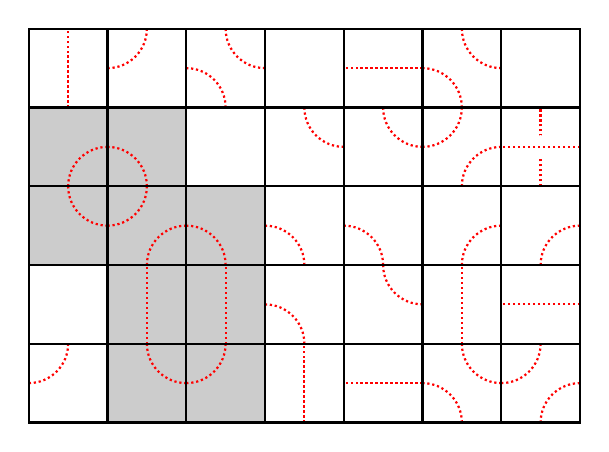
\begin{tikzpicture}
    % row1
    \cellD{0}{0}{1}{1}
    \cellCf{1}{0}{2}{1}
    \cellDf{2}{0}{3}{1}
    \cellF{3}{0}{4}{1}
    \cellE{4}{0}{5}{1}
    \cellG{5}{0}{6}{1}
    \cellH{6}{0}{7}{1}
    % row2
    \cell{0}{1}{1}{2}
    \cellFf{1}{1}{2}{2}
    \cellFf{2}{1}{3}{2}
    \cellA{3}{1}{4}{2}
    \cellC{4}{1}{5}{2}
    \cellF{5}{1}{6}{2}
    \cellE{6}{1}{7}{2}
    % row3
    \cellCf{0}{2}{1}{3}
    \cellHf{1}{2}{2}{3}
    \cellAf{2}{2}{3}{3}
    \cellA{3}{2}{4}{3}
    \cellA{4}{2}{5}{3}
    \cellB{5}{2}{6}{3}
    \cellB{6}{2}{7}{3}
    % row4
    \cellBf{0}{3}{1}{4}
    \cellAf{1}{3}{2}{4}
    \cell{2}{3}{3}{4}
    \cellC{3}{3}{4}{4}
    \cellC{4}{3}{5}{4}
    \cellH{5}{3}{6}{4}
    \cellI{6}{3}{7}{4}
    % row5
    \cellF{0}{4}{1}{5}
    \cellD{1}{4}{2}{5}
    \cellG{2}{4}{3}{5}
    \cell{3}{4}{4}{5}
    \cellE{4}{4}{5}{5}
    \cellG{5}{4}{6}{5}
    \cell{6}{4}{7}{5}
\end{tikzpicture}

\end{center}
\caption{A messy knot mosaic with $1$ knot}
\label{fig:messy multi knot}
\end{figure}

\end{exmp}

\section{A ``Per-Cell" Identity}

Though Equation \ref{eq:ugly inc excl} does compute $s_{m,n}$, the $K$ function is a function that references the entire, global structure of $\ell$. It is useful to recover the $(-1)^{K(\ell)}$ term using only ``per-cell", local information.

\begin{prop}
    Let $\mathcal{K}$ be the set of cells in a binary lattice $\ell$ that specify a knot.
    
    There exists $p_{(i,j)} \in \{-1,1\}$ so that

    \begin{equation}
        \prod_{\text{Cell } (i,j) \in \mathcal{K}} p_{(i,j)} = -1
        \label{eq:neg prod knot condition}
    \end{equation}

    for all possible $\mathcal{K}$.
    \label{prop:neg prod prop}
\end{prop}

\begin{proof}
    \textbf{TODO}
\end{proof}

Proposition \ref{prop:neg prod prop} allows us to rewrite the term in the sum of Equation \ref{eq:ugly inc excl} to

\begin{equation}
    (-1)^{K(\ell)}U(\ell) = (-1)^{K(\ell)} \prod_{\text{Cell }(i,j) \in \ell} u_{(i,j)} = \prod_{\text{Cell }(i,j) \in \ell} p_{(i,j)}u_{(i,j)} \text{ $\forall \ell$}.
    \label{eq:term fix}
\end{equation}

We summarize the values of $v_{(i,j)} := p_{(i,j)}u_{(i,j)}$ in Table \ref{tbl:values of p and v}.

\begin{table}[h!]
    \begin{center}
        \begin{tabular}{ |c|r|r|r|c|r|r|r| } 
            \hline
            \textbf{Cell (}$\mathbf{i}$\textbf{,} $\mathbf{j}$\textbf{)} & $\mathbf{u_{(i,j)}}$ & $\mathbf{p_{(i,j)}}$ & $\mathbf{v_{(i,j)}}$ & \textbf{Cell (}$\mathbf{i}$\textbf{,} $\mathbf{j}$\textbf{)} & $\mathbf{u_{(i,j)}}$ & $\mathbf{p_{(i,j)}}$ & $\mathbf{v_{(i,j)}}$ \\ 
            \hline
            $(00, 00)$ & $11$ & $1$ & $11$ & $(10, 00)$ & $1$ & $-1$ & $-1$ \\
            \hline
            $(00, 01)$ & $1$ & $1$ & $1$ & $(10, 01)$ & $4$ & $1$ & $4$ \\
            \hline
            $(00, 10)$ & $1$ & $1$ & $1$ & $(10, 10)$ & $1$ & $1$ & $1$ \\
            \hline
            $(00, 11)$ & $1$ & $1$ & $1$ & $(10, 11)$ & $1$ & $1$ & $1$ \\
            \hline
            $(01, 00)$ & $1$ & $1$ & $1$ & $(11, 00)$ & $1$ & $1$ & $1$ \\
            \hline
            $(01, 01)$ & $1$ & $1$ & $1$ & $(11, 01)$ & $1$ & $1$ & $1$ \\
            \hline
            $(01, 10)$ & $4$ & $-1$ & $-4$ & $(11, 10)$ & $1$ & $-1$ & $-1$ \\
            \hline
            $(01, 11)$ & $1$ & $1$ & $1$ & $(11, 11)$ & $11$ & $1$ & $11$ \\
            \hline
        \end{tabular}
        \caption{Values of $p_{(i,j)}$ and $v_{(i,j)}$}
        \label{tbl:values of p and v}
    \end{center}
\end{table}

Equation \ref{eq:term fix} allows us to simplify Equation \ref{eq:ugly inc excl} to

\begin{equation}
    s_{m,n} = \sum_{\ell \in \mathbb{L}^{(m,n)}} \prod_{\text{Cell }(i,j) \in \ell} v_{(i,j)}.
\label{eq:technically correct}
\end{equation}

$s_{m,n}$ can be calculated more efficiently than in Equation \ref{eq:technically correct} using the state matrix recursion introduced in Theorem \ref{thm:Oh2014}.

\section{Proof of Theorem \ref{thm: messy mosaics}}



\textbf{TODO} induction and definition for state matrix

\textbf{TODO} induction for matrix powers


\textbf{TODO} complexity 

Equation \ref{eq:technically correct} has $mn 2^{(m-1)(n-1)}$ multiplications.

Theorem \ref{thm: messy mosaics} uses $4^2 + 4^3 + 4^4 + 4^{m-1} = 4^2 \frac{4^{m-2}-1}{4-1}$ multiplications for the construction of $A(m)$, and using the naive matrix multiplication algorithm we have ${2^{3(m-1)}}\left\lceil \log_2(n) \right\rceil$ multiplications to compute $A(m)^n$.

If we set $m=n$, calculating $s_{m,m}$ with Equation \ref{eq:technically correct} is $O(m^2 2^{m^2})$, while Theorem \ref{thm: messy mosaics} is $O(\log(m)8^m)$.

\section{OLD STUFF}

\begin{proof}
We consider the same vertex labeling in the proof of Theorem \ref{thm: main theorem}, namely labeling a vertex by the number of polygons that contain it $\text{mod } 2$. Though avoided in the previous proof for clarity, it is important to think of each individual cell labeling as having its own weight, which corresponds with how many distinct tiles can map to the cell labeling.

\begin{center}
    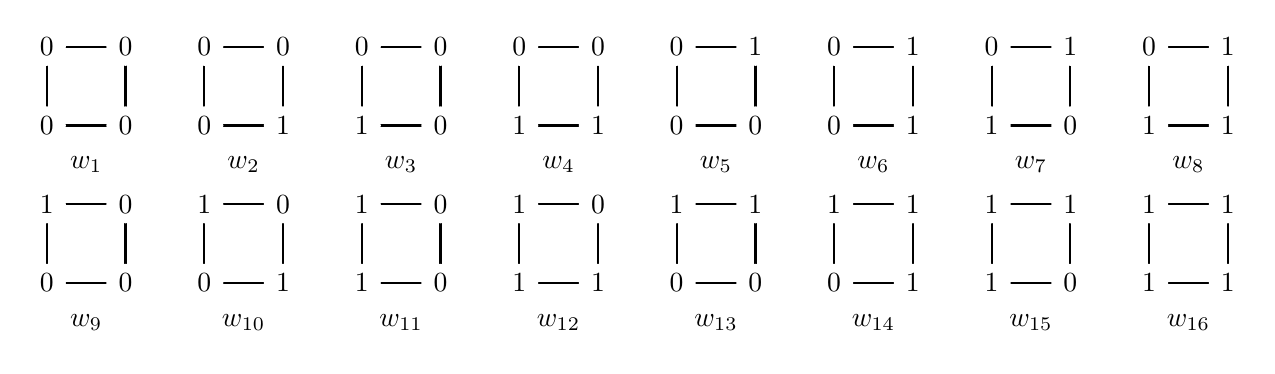
\begin{tikzpicture}
        % row1
        \cell{0}{0}{1}{1}
        \cell{2}{0}{3}{1}
        \cell{4}{0}{5}{1}
        \cell{6}{0}{7}{1}
        \cell{8}{0}{9}{1}
        \cell{10}{0}{11}{1}
        \cell{12}{0}{13}{1}
        \cell{14}{0}{15}{1}
        % row2
        \cell{0}{2}{1}{3}
        \cell{2}{2}{3}{3}
        \cell{4}{2}{5}{3}
        \cell{6}{2}{7}{3}
        \cell{8}{2}{9}{3}
        \cell{10}{2}{11}{3}
        \cell{12}{2}{13}{3}
        \cell{14}{2}{15}{3}

        % label for row1
        \( \lablvertex{0}{0}{$0$} \)
        \( \lablvertex{1}{0}{$0$} \)
        \( \lablvertex{2}{0}{$0$} \)
        \( \lablvertex{3}{0}{$1$} \)
        \( \lablvertex{4}{0}{$1$} \)
        \( \lablvertex{5}{0}{$0$} \)
        \( \lablvertex{6}{0}{$1$} \)
        \( \lablvertex{7}{0}{$1$} \)
        \( \lablvertex{8}{0}{$0$} \)
        \( \lablvertex{9}{0}{$0$} \)
        \( \lablvertex{10}{0}{$0$} \)
        \( \lablvertex{11}{0}{$1$} \)
        \( \lablvertex{12}{0}{$1$} \)
        \( \lablvertex{13}{0}{$0$} \)
        \( \lablvertex{14}{0}{$1$} \)
        \( \lablvertex{15}{0}{$1$} \)
        
        % label for row1
        \( \lablvertex{0}{1}{$1$} \)
        \( \lablvertex{1}{1}{$0$} \)
        \( \lablvertex{2}{1}{$1$} \)
        \( \lablvertex{3}{1}{$0$} \)
        \( \lablvertex{4}{1}{$1$} \)
        \( \lablvertex{5}{1}{$0$} \)
        \( \lablvertex{6}{1}{$1$} \)
        \( \lablvertex{7}{1}{$0$} \)
        \( \lablvertex{8}{1}{$1$} \)
        \( \lablvertex{9}{1}{$1$} \)
        \( \lablvertex{10}{1}{$1$} \)
        \( \lablvertex{11}{1}{$1$} \)
        \( \lablvertex{12}{1}{$1$} \)
        \( \lablvertex{13}{1}{$1$} \)
        \( \lablvertex{14}{1}{$1$} \)
        \( \lablvertex{15}{1}{$1$} \)

        \( \lablvertex{0}{2}{$0$} \)
        \( \lablvertex{1}{2}{$0$} \)
        \( \lablvertex{2}{2}{$0$} \)
        \( \lablvertex{3}{2}{$1$} \)
        \( \lablvertex{4}{2}{$1$} \)
        \( \lablvertex{5}{2}{$0$} \)
        \( \lablvertex{6}{2}{$1$} \)
        \( \lablvertex{7}{2}{$1$} \)
        \( \lablvertex{8}{2}{$0$} \)
        \( \lablvertex{9}{2}{$0$} \)
        \( \lablvertex{10}{2}{$0$} \)
        \( \lablvertex{11}{2}{$1$} \)
        \( \lablvertex{12}{2}{$1$} \)
        \( \lablvertex{13}{2}{$0$} \)
        \( \lablvertex{14}{2}{$1$} \)
        \( \lablvertex{15}{2}{$1$} \)

        \( \lablvertex{0}{3}{$0$} \)
        \( \lablvertex{1}{3}{$0$} \)
        \( \lablvertex{2}{3}{$0$} \)
        \( \lablvertex{3}{3}{$0$} \)
        \( \lablvertex{4}{3}{$0$} \)
        \( \lablvertex{5}{3}{$0$} \)
        \( \lablvertex{6}{3}{$0$} \)
        \( \lablvertex{7}{3}{$0$} \)
        \( \lablvertex{8}{3}{$0$} \)
        \( \lablvertex{9}{3}{$1$} \)
        \( \lablvertex{10}{3}{$0$} \)
        \( \lablvertex{11}{3}{$1$} \)
        \( \lablvertex{12}{3}{$0$} \)
        \( \lablvertex{13}{3}{$1$} \)
        \( \lablvertex{14}{3}{$0$} \)
        \( \lablvertex{15}{3}{$1$} \)

        % numbers row 1
        \( \lablnode{0.5}{-0.5}{$w_{9}$} \)
        \( \lablnode{2.5}{-0.5}{$w_{10}$} \)
        \( \lablnode{4.5}{-0.5}{$w_{11}$} \)
        \( \lablnode{6.5}{-0.5}{$w_{12}$} \)
        \( \lablnode{8.5}{-0.5}{$w_{13}$} \)
        \( \lablnode{10.5}{-0.5}{$w_{14}$} \)
        \( \lablnode{12.5}{-0.5}{$w_{15}$} \)
        \( \lablnode{14.5}{-0.5}{$w_{16}$} \)
        % numbers row 2
        \( \lablnode{0.5}{1.5}{$w_{1}$} \)
        \( \lablnode{2.5}{1.5}{$w_{2}$} \)
        \( \lablnode{4.5}{1.5}{$w_{3}$} \)
        \( \lablnode{6.5}{1.5}{$w_{4}$} \)
        \( \lablnode{8.5}{1.5}{$w_{5}$} \)
        \( \lablnode{10.5}{1.5}{$w_{6}$} \)
        \( \lablnode{12.5}{1.5}{$w_{7}$} \)
        \( \lablnode{14.5}{1.5}{$w_{8}$} \)
    \end{tikzpicture}
\end{center}

The proof of Theorem \ref{thm: main theorem} can be seen as assigning $w_{7} = w_{10} = 0$, and all other weights to $1$. The usefulness of this view can be seen when considering the operation for creating the recursive definition for $A(k)$ in the previous proof. Previously, we defined the coefficient matrix $V$ by computing $A(2)$ and $A(3)$ directly and comparing. Now with a weight assigned to individual cell labelings, we can define the values of $A(2)$ and $V$ directly in terms of these weights.

$$
A(2) = 
\begin{bmatrix}
    w_{1}w_{1} & w_{2} w_{5} \\
    w_{3} w_{9} & w_{4} w_{13}
\end{bmatrix},
V = 
\begin{bmatrix}
    \frac{w_{1} w_{1}}{w_{1}} & \frac{w_{2} w_{5}}{w_{1}} & \frac{w_{1} w_{2}}{w_{2}} & \frac{w_{2} w_{6}}{w_{2}} \\
    \frac{w_{3} w_{9}}{w_{1}} & \frac{w_{4} w_{13}}{w_{1}} & \frac{w_{3} w_{10}}{w_{2}} & \frac{w_{4} w_{14}}{w_{2}} \\
    \frac{w_{1} w_{3}}{w_{3}} & \frac{w_{2} w_{7}}{w_{3}} & \frac{w_{1} w_{4}}{w_{4}} & \frac{w_{2} w_{8}}{w_{4}} \\
    \frac{w_{3} w_{11}}{w_{3}} & \frac{w_{4} w_{15}}{w_{3}} & \frac{w_{3} w_{12}}{w_{4}} & \frac{w_{4} w_{16}}{w_{4}}
\end{bmatrix}
= 
\begin{bmatrix}
    w_{1} & \frac{w_{2} w_{5}}{w_{1}} & w_{1} & w_{6} \\
    \frac{w_{3} w_{9}}{w_{1}} & \frac{w_{4} w_{13}}{w_{1}} & \frac{w_{3} w_{10}}{w_{2}} & \frac{w_{4} w_{14}}{w_{2}} \\
    w_{1} & \frac{w_{2} w_{7}}{w_{3}} & w_{1} & \frac{w_{2} w_{8}}{w_{4}} \\
    w_{11} & \frac{w_{4} w_{15}}{w_{3}} & \frac{w_{3} w_{12}}{w_{4}} & w_{16}
\end{bmatrix}.
$$

With this identity, we can enumerate $t_{m,n}$ once we have proper assignments for the $16$ weights. As in the previous proof, we have $w_{7}=w_{10}=0$, as again these are impossible vertex labelings for our tile set. 

Next consider the cell labelings for $w_{1}$ and $w_{16}$. When enumerating polygon mosaics (and their messy variant), these cell labelings do not contribute to the cells of a polygon. For polygon mosaics, only the $T_1$ tile are permitted to not contribute to the shape of a polygon. However, in messy polygon mosaics, all $7$ tiles are permitted to not contribute to the shape of the polygon, so $w_{1} = w_{16}=7$.

However, this means we now lose the uniqueness of the map from vertex labeling to messy polygon mosaics. For instance, the sub-grid vertex labelings below are now ambiguous as to whether or not they represent a polygon.

\begin{center}
    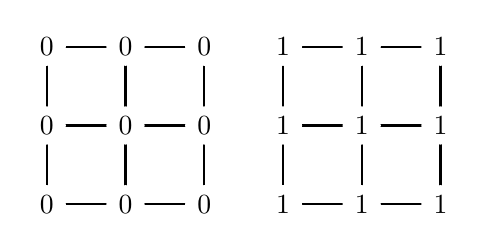
\begin{tikzpicture}
        % row1
        \cell{0}{0}{1}{1}
        \cell{0}{1}{1}{2}
        \cell{1}{0}{2}{1}
        \cell{1}{1}{2}{2}

        \( \lablvertex{0}{0}{$0$} \)
        \( \lablvertex{1}{0}{$0$} \)
        \( \lablvertex{2}{0}{$0$} \)

        \( \lablvertex{0}{1}{$0$} \)
        \( \lablvertex{1}{1}{$0$} \)
        \( \lablvertex{2}{1}{$0$} \)
        
        \( \lablvertex{0}{2}{$0$} \)
        \( \lablvertex{1}{2}{$0$} \)
        \( \lablvertex{2}{2}{$0$} \)
        
        % row1
        \cell{3}{0}{4}{1}
        \cell{3}{1}{4}{2}
        \cell{4}{0}{5}{1}
        \cell{4}{1}{5}{2}

        \( \lablvertex{3}{0}{$1$} \)
        \( \lablvertex{4}{0}{$1$} \)
        \( \lablvertex{5}{0}{$1$} \)

        \( \lablvertex{3}{1}{$1$} \)
        \( \lablvertex{4}{1}{$1$} \)
        \( \lablvertex{5}{1}{$1$} \)

        \( \lablvertex{3}{2}{$1$} \)
        \( \lablvertex{4}{2}{$1$} \)
        \( \lablvertex{5}{2}{$1$} \)

    \end{tikzpicture}
\end{center}

This ambiguity is explored in the following example.

\begin{exmp}\label{exmp: iep}

Consider the four vertex labelings below, along with the messy polygon mosaic on the right. Write the product of the weights of all cell labelings below each, assuming all weights not defined above are $1$.

\begin{center}
    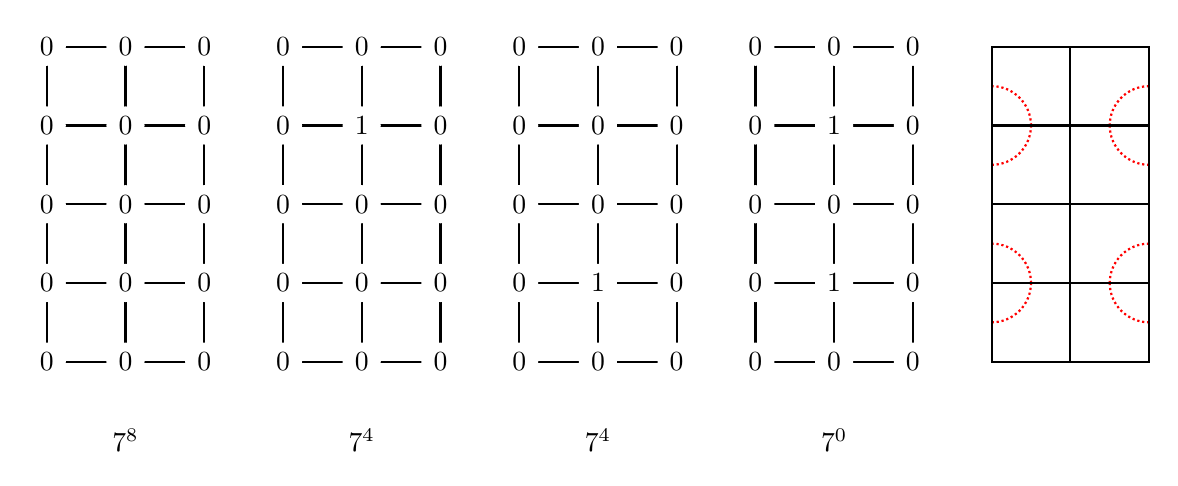
\begin{tikzpicture}
        % row1
        \cell{-6}{0}{-5}{1}
        \cell{-6}{1}{-5}{2}
        \cell{-6}{2}{-5}{3}
        \cell{-6}{3}{-5}{4}
        \cell{-5}{0}{-4}{1}
        \cell{-5}{1}{-4}{2}
        \cell{-5}{2}{-4}{3}
        \cell{-5}{3}{-4}{4}

        \( \lablnode{-5}{-1}{$7^8$} \)

        \( \lablvertex{-6}{0}{$0$} \)
        \( \lablvertex{-5}{0}{$0$} \)
        \( \lablvertex{-4}{0}{$0$} \)

        \( \lablvertex{-6}{1}{$0$} \)
        \( \lablvertex{-5}{1}{$0$} \)
        \( \lablvertex{-4}{1}{$0$} \)

        \( \lablvertex{-6}{2}{$0$} \)
        \( \lablvertex{-5}{2}{$0$} \)
        \( \lablvertex{-4}{2}{$0$} \)

        \( \lablvertex{-6}{3}{$0$} \)
        \( \lablvertex{-5}{3}{$0$} \)
        \( \lablvertex{-4}{3}{$0$} \)

        \( \lablvertex{-6}{4}{$0$} \)
        \( \lablvertex{-5}{4}{$0$} \)
        \( \lablvertex{-4}{4}{$0$} \)
        % row1
        \cell{-3}{0}{-2}{1}
        \cell{-3}{1}{-2}{2}
        \cell{-3}{2}{-2}{3}
        \cell{-3}{3}{-2}{4}
        \cell{-2}{0}{-1}{1}
        \cell{-2}{1}{-1}{2}
        \cell{-2}{2}{-1}{3}
        \cell{-2}{3}{-1}{4}

        \( \lablnode{-2}{-1}{$7^4$} \)

        \( \lablvertex{-3}{0}{$0$} \)
        \( \lablvertex{-2}{0}{$0$} \)
        \( \lablvertex{-1}{0}{$0$} \)

        \( \lablvertex{-3}{1}{$0$} \)
        \( \lablvertex{-2}{1}{$0$} \)
        \( \lablvertex{-1}{1}{$0$} \)

        \( \lablvertex{-3}{2}{$0$} \)
        \( \lablvertex{-2}{2}{$0$} \)
        \( \lablvertex{-1}{2}{$0$} \)

        \( \lablvertex{-3}{3}{$0$} \)
        \( \lablvertex{-2}{3}{$1$} \)
        \( \lablvertex{-1}{3}{$0$} \)

        \( \lablvertex{-3}{4}{$0$} \)
        \( \lablvertex{-2}{4}{$0$} \)
        \( \lablvertex{-1}{4}{$0$} \)

        % row1
        \cell{0}{0}{1}{1}
        \cell{0}{1}{1}{2}
        \cell{0}{2}{1}{3}
        \cell{0}{3}{1}{4}
        \cell{1}{0}{2}{1}
        \cell{1}{1}{2}{2}
        \cell{1}{2}{2}{3}
        \cell{1}{3}{2}{4}

        \( \lablnode{1}{-1}{$7^4$} \)
        
        \( \lablvertex{0}{0}{$0$} \)
        \( \lablvertex{1}{0}{$0$} \)
        \( \lablvertex{2}{0}{$0$} \)

        \( \lablvertex{0}{1}{$0$} \)
        \( \lablvertex{1}{1}{$1$} \)
        \( \lablvertex{2}{1}{$0$} \)

        \( \lablvertex{0}{2}{$0$} \)
        \( \lablvertex{1}{2}{$0$} \)
        \( \lablvertex{2}{2}{$0$} \)

        \( \lablvertex{0}{3}{$0$} \)
        \( \lablvertex{1}{3}{$0$} \)
        \( \lablvertex{2}{3}{$0$} \)

        \( \lablvertex{0}{4}{$0$} \)
        \( \lablvertex{1}{4}{$0$} \)
        \( \lablvertex{2}{4}{$0$} \)

        % row1
        \cell{3}{0}{4}{1}
        \cell{3}{1}{4}{2}
        \cell{3}{2}{4}{3}
        \cell{3}{3}{4}{4}
        \cell{4}{0}{5}{1}
        \cell{4}{1}{5}{2}
        \cell{4}{2}{5}{3}
        \cell{4}{3}{5}{4}

        \( \lablnode{4}{-1}{$7^0$} \)

        \( \lablvertex{3}{0}{$0$} \)
        \( \lablvertex{4}{0}{$0$} \)
        \( \lablvertex{5}{0}{$0$} \)

        \( \lablvertex{3}{1}{$0$} \)
        \( \lablvertex{4}{1}{$1$} \)
        \( \lablvertex{5}{1}{$0$} \)

        \( \lablvertex{3}{2}{$0$} \)
        \( \lablvertex{4}{2}{$0$} \)
        \( \lablvertex{5}{2}{$0$} \)

        \( \lablvertex{3}{3}{$0$} \)
        \( \lablvertex{4}{3}{$1$} \)
        \( \lablvertex{5}{3}{$0$} \)

        \( \lablvertex{3}{4}{$0$} \)
        \( \lablvertex{4}{4}{$0$} \)
        \( \lablvertex{5}{4}{$0$} \)

        \cellD{6}{0}{7}{1}
        \cellC{7}{0}{8}{1}

        \cellA{6}{1}{7}{2}
        \cellB{7}{1}{8}{2}

        \cellD{6}{2}{7}{3}
        \cellC{7}{2}{8}{3}    

        \cellA{6}{3}{7}{4}
        \cellB{7}{3}{8}{4}    

    \end{tikzpicture}
\end{center}

Notice that each vertex labeling could include the right-most messy polygon mosaic. In fact, the left-most vertex labeling contains all possible mosaics! If we were to add these weight products together, we would count the right messy polygon mosaic $4$ times.

\end{exmp}

The double counting demonstrated in Example \ref{exmp: iep} motivates the following idea. If vertex labelings with an odd number of polygons are negative, then the addition of these weight products would incorporate the \textit{inclusion-exclusion principle}, mitigating the double counting. In Example \ref{exmp: iep}, the sum $7^8 - 7^4 - 7^4 + 7^0$ would then represent the number of mosaics that \textit{do not} contain the following three classes of messy polygon mosaics, where cells that can be any tile are marked with a dot.

\begin{center}
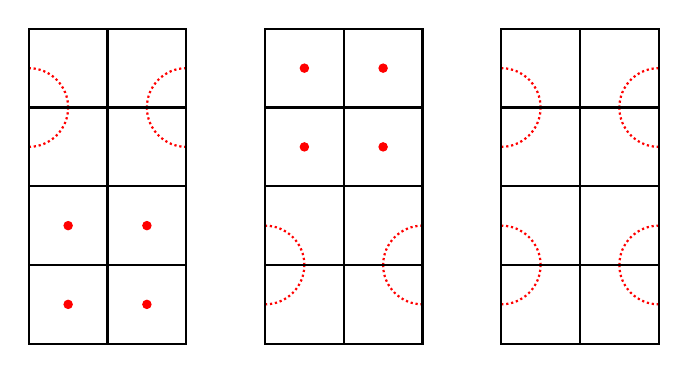
\begin{tikzpicture}
    %
    \cellopen{0}{0}{1}{1}
    \cellopen{1}{0}{2}{1}

    \cellopen{0}{1}{1}{2}
    \cellopen{1}{1}{2}{2}

    \cellD{0}{2}{1}{3}
    \cellC{1}{2}{2}{3}    

    \cellA{0}{3}{1}{4}
    \cellB{1}{3}{2}{4}
    %
    \cellD{3}{0}{4}{1}
    \cellC{4}{0}{5}{1}

    \cellA{3}{1}{4}{2}
    \cellB{4}{1}{5}{2}

    \cellopen{3}{2}{4}{3}
    \cellopen{4}{2}{5}{3}    

    \cellopen{3}{3}{4}{4}
    \cellopen{4}{3}{5}{4}
    %
    \cellD{6}{0}{7}{1}
    \cellC{7}{0}{8}{1}

    \cellA{6}{1}{7}{2}
    \cellB{7}{1}{8}{2}

    \cellD{6}{2}{7}{3}
    \cellC{7}{2}{8}{3}    

    \cellA{6}{3}{7}{4}
    \cellB{7}{3}{8}{4}
\end{tikzpicture}
\end{center}

Therefore, the sum over the products for all vertex labelings, where the product is negative if the vertex labeling represents an odd number of polygons in the mosaic, would be the number of mosaics that \textit{do not} include messy polygon mosaics.

We can accomplish this by finding a weight assignment such that the product over the cell labeling weights of \textit{any} single polygon equals $-1$. It is not obvious that such an assignment can even be found! 

Luckily such assignments exist. The proof of this fact can be found in the Appendix, and choosing an assignment gives us the following weight assignments.

\begin{center}
    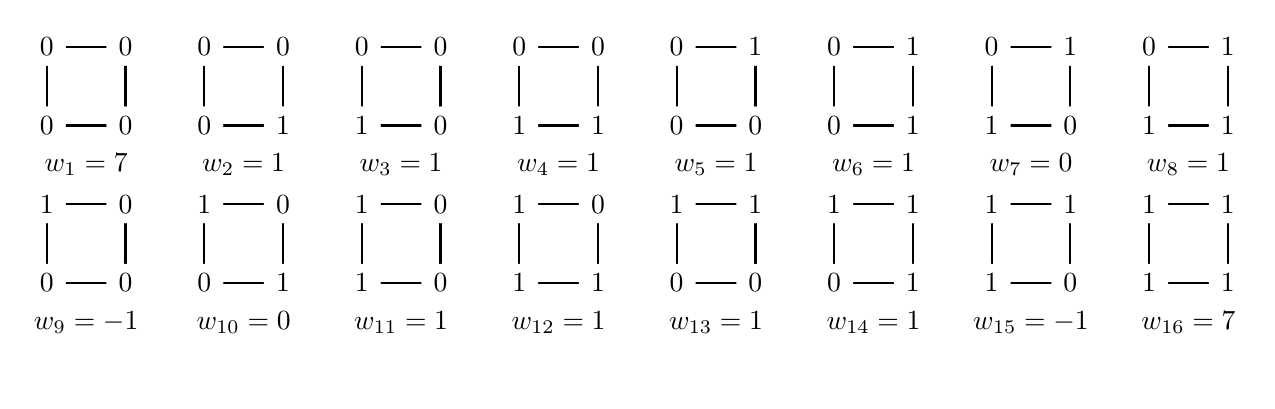
\begin{tikzpicture}
        % row1
        \cell{0}{0}{1}{1}
        \cell{2}{0}{3}{1}
        \cell{4}{0}{5}{1}
        \cell{6}{0}{7}{1}
        \cell{8}{0}{9}{1}
        \cell{10}{0}{11}{1}
        \cell{12}{0}{13}{1}
        \cell{14}{0}{15}{1}
        % row2
        \cell{0}{2}{1}{3}
        \cell{2}{2}{3}{3}
        \cell{4}{2}{5}{3}
        \cell{6}{2}{7}{3}
        \cell{8}{2}{9}{3}
        \cell{10}{2}{11}{3}
        \cell{12}{2}{13}{3}
        \cell{14}{2}{15}{3}

        % label for row1
        \( \lablvertex{0}{0}{$0$} \)
        \( \lablvertex{1}{0}{$0$} \)
        \( \lablvertex{2}{0}{$0$} \)
        \( \lablvertex{3}{0}{$1$} \)
        \( \lablvertex{4}{0}{$1$} \)
        \( \lablvertex{5}{0}{$0$} \)
        \( \lablvertex{6}{0}{$1$} \)
        \( \lablvertex{7}{0}{$1$} \)
        \( \lablvertex{8}{0}{$0$} \)
        \( \lablvertex{9}{0}{$0$} \)
        \( \lablvertex{10}{0}{$0$} \)
        \( \lablvertex{11}{0}{$1$} \)
        \( \lablvertex{12}{0}{$1$} \)
        \( \lablvertex{13}{0}{$0$} \)
        \( \lablvertex{14}{0}{$1$} \)
        \( \lablvertex{15}{0}{$1$} \)
        
        % label for row1
        \( \lablvertex{0}{1}{$1$} \)
        \( \lablvertex{1}{1}{$0$} \)
        \( \lablvertex{2}{1}{$1$} \)
        \( \lablvertex{3}{1}{$0$} \)
        \( \lablvertex{4}{1}{$1$} \)
        \( \lablvertex{5}{1}{$0$} \)
        \( \lablvertex{6}{1}{$1$} \)
        \( \lablvertex{7}{1}{$0$} \)
        \( \lablvertex{8}{1}{$1$} \)
        \( \lablvertex{9}{1}{$1$} \)
        \( \lablvertex{10}{1}{$1$} \)
        \( \lablvertex{11}{1}{$1$} \)
        \( \lablvertex{12}{1}{$1$} \)
        \( \lablvertex{13}{1}{$1$} \)
        \( \lablvertex{14}{1}{$1$} \)
        \( \lablvertex{15}{1}{$1$} \)

        \( \lablvertex{0}{2}{$0$} \)
        \( \lablvertex{1}{2}{$0$} \)
        \( \lablvertex{2}{2}{$0$} \)
        \( \lablvertex{3}{2}{$1$} \)
        \( \lablvertex{4}{2}{$1$} \)
        \( \lablvertex{5}{2}{$0$} \)
        \( \lablvertex{6}{2}{$1$} \)
        \( \lablvertex{7}{2}{$1$} \)
        \( \lablvertex{8}{2}{$0$} \)
        \( \lablvertex{9}{2}{$0$} \)
        \( \lablvertex{10}{2}{$0$} \)
        \( \lablvertex{11}{2}{$1$} \)
        \( \lablvertex{12}{2}{$1$} \)
        \( \lablvertex{13}{2}{$0$} \)
        \( \lablvertex{14}{2}{$1$} \)
        \( \lablvertex{15}{2}{$1$} \)

        \( \lablvertex{0}{3}{$0$} \)
        \( \lablvertex{1}{3}{$0$} \)
        \( \lablvertex{2}{3}{$0$} \)
        \( \lablvertex{3}{3}{$0$} \)
        \( \lablvertex{4}{3}{$0$} \)
        \( \lablvertex{5}{3}{$0$} \)
        \( \lablvertex{6}{3}{$0$} \)
        \( \lablvertex{7}{3}{$0$} \)
        \( \lablvertex{8}{3}{$0$} \)
        \( \lablvertex{9}{3}{$1$} \)
        \( \lablvertex{10}{3}{$0$} \)
        \( \lablvertex{11}{3}{$1$} \)
        \( \lablvertex{12}{3}{$0$} \)
        \( \lablvertex{13}{3}{$1$} \)
        \( \lablvertex{14}{3}{$0$} \)
        \( \lablvertex{15}{3}{$1$} \)

        % numbers row 1
        \( \lablnode{0.5}{-0.5}{$w_{9}=-1$} \)
        \( \lablnode{2.5}{-0.5}{$w_{10}=0$} \)
        \( \lablnode{4.5}{-0.5}{$w_{11}=1$} \)
        \( \lablnode{6.5}{-0.5}{$w_{12}=1$} \)
        \( \lablnode{8.5}{-0.5}{$w_{13}=1$} \)
        \( \lablnode{10.5}{-0.5}{$w_{14}=1$} \)
        \( \lablnode{12.5}{-0.5}{$w_{15}=-1$} \)
        \( \lablnode{14.5}{-0.5}{$w_{16}=7$} \)
        % numbers row 2
        \( \lablnode{0.5}{1.5}{$w_{1}=7$} \)
        \( \lablnode{2.5}{1.5}{$w_{2}=1$} \)
        \( \lablnode{4.5}{1.5}{$w_{3}=1$} \)
        \( \lablnode{6.5}{1.5}{$w_{4}=1$} \)
        \( \lablnode{8.5}{1.5}{$w_{5}=1$} \)
        \( \lablnode{10.5}{1.5}{$w_{6}=1$} \)
        \( \lablnode{12.5}{1.5}{$w_{7}=0$} \)
        \( \lablnode{14.5}{1.5}{$w_{8}=1$} \)
    \end{tikzpicture}
\end{center}

This immediately gives us a way to construct an analagous definition for $A(k+1)$ given $A(k)$. Once we write $A(k) = \begin{bmatrix} A_{0,0} & A_{0,1} \\ A_{1,0} & A_{1,1} \end{bmatrix}$, we have

$$
A(2) = 
\begin{bmatrix}
    7^2 & 1 \\
    -1 & 1
\end{bmatrix},
V = 
\begin{bmatrix}
    7 & \frac{1}{7} & 7 & 1 \\
    -\frac{1}{7} & 1 & 0 & 1 \\
    7 & 0 & 7  & 1 \\
    1 & -1 & 1 & 7 \\
\end{bmatrix}
$$

Subsituting $V$ into Equation \ref{eqn: coefficient matrix prod} gives the result.

\end{proof}


\section{Extensions}
\label{section: Extensions}

Hong and Oh \cite{Hong2018} study the mosaic system with the tile set $\mathbb{T}^* = \{T_0, \dots,T_7\}$. This tile set constructs shapes we call \textit{polygons}\footnote{Polygons are more commonly called "self-avoiding polygons" in the literature to emphasize their relationship with self-avoiding walks.}. If we let $p_{m,n}$ be the number of polygon mosaics of size $(m,n)$, Hong and Oh showed the following results\footnote{The authors did not consider the mosaic containing all $T_0$ tiles a polygon mosaic, and so define $p_{m,n}$ as one less than what we define.}. 

\begin{thm}[\cite{Hong2018}]
    \label{thm:Hong2018}
    The number of polygon mosaics of size $(m,n)$ $p_{m,n}$ for $m,n \geq 2$ has

    $$2^{m+n-3} \left(\frac{17}{10}\right)^{(m-2)(n-2)} \leq p_{m,n} \leq 2^{m+n-3} \left(\frac{31}{16}\right)^{(m-2)(n-2)}.$$
\end{thm}

Though not stated in Hong and Oh \cite{Hong2018}, $p_{m,n}$ is exactly enumerated by Theorem \ref{thm:Oh2014} by replacing the $4$ in the definition of $O_{k+1}$ with a $0$.The array $p_{n,m}$ is A181245 on the OEIS \cite[OEIS]{oeis}. 

\textbf{TODO}

\section{Acknowledgements}

The authors would like to thank Michael Maltenfort for the edits, improvements and ideas for this paper. 

\printbibliography


\section{Appendix}

We demonstrate that weight assignments exist such that the product over the cell labeling weights of \textit{all} single polygons equals $-1$. We do this by first asserting that the product of the weights associated with the smallest polygon multiply to $-1$, ie. $w_2 w_3 w_5 w_9 = -1$. 

\begin{lemma}\label{lemma: build bigger saps}
    One can construct all larger polygons from the smallest polygon using a finite set of transformations $S$.
\end{lemma}

\begin{proof}
    TODO Something about changing vertex values
\end{proof}

This is because one can find $w_{1} , \dots, w_{16}$ so that the following two constraints hold:

\begin{constraint}\label{constraint: smallest sap prod}
    The weights associated with the smallest polygon multiply to $-1$, ie. $w_2 w_3 w_5 w_9 = -1.$ 
\end{constraint}

\begin{constraint}\label{constraint: prod works}
    All transformations in $S$ preserve the weight product of a changed polygon.
\end{constraint}

Constraint \ref{constraint: smallest sap prod} and Constraint \ref{constraint: prod works} amount to a series of constraints on the values of $w_i$. Choosing a solution set from these constraints gives the following weights.

Flipping the parity of a single vertex in a vertex labeling changes the $4$ surrounding cells. This creates a constraint on a subset of $w_1 ,\dots, w_{16}.$ 

The flipping of parity of a single vertex results in $2$ distinct types of constraints. Let a constraint of \textit{Type 1} be a parity flip that does not change the number of polygons represented in the vertex labeling. For example, consider the following flip of the center vertex in the following sub vertex labeling.

\begin{center}
    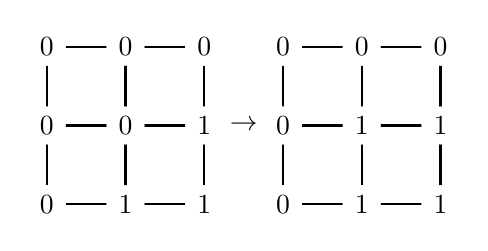
\begin{tikzpicture}
        % row1
        \cell{0}{0}{1}{1}
        \cell{1}{0}{2}{1}
        % row2
        \cell{0}{1}{1}{2}
        \cell{1}{1}{2}{2}
        % label for row1
        \( \lablvertex{0}{0}{$0$} \)
        \( \lablvertex{1}{0}{$1$} \)
        \( \lablvertex{2}{0}{$1$} \)
        % label for row2
        \( \lablvertex{0}{1}{$0$} \)
        \( \lablvertex{1}{1}{$0$} \)
        \( \lablvertex{2}{1}{$1$} \)
        % label for row3
        \( \lablvertex{0}{2}{$0$} \)
        \( \lablvertex{1}{2}{$0$} \)
        \( \lablvertex{2}{2}{$0$} \)
        % row1
        \cell{3}{0}{4}{1}
        \cell{4}{0}{5}{1}
        % row2
        \cell{3}{1}{4}{2}
        \cell{4}{1}{5}{2}
        % label for row1
        \( \lablvertex{3}{0}{$0$} \)
        \( \lablvertex{4}{0}{$1$} \)
        \( \lablvertex{5}{0}{$1$} \)
        % label for row2
        \( \lablvertex{3}{1}{$0$} \)
        \( \lablvertex{4}{1}{$1$} \)
        \( \lablvertex{5}{1}{$1$} \)
        % label for row3
        \( \lablvertex{3}{2}{$0$} \)
        \( \lablvertex{4}{2}{$0$} \)
        \( \lablvertex{5}{2}{$0$} \)

        \( \lablnode{2.5}{1}{$\rightarrow$} \)
    \end{tikzpicture}
\end{center}

As this does not change the associated number of polygons in the larger vertex labeling, we want this to preserve the sign of the weight product. This gives the following associated constraint. 

$$\text{sign}(w_{1}w_{2}w_{5}w_{9}) = \text{sign}(w_{2}w_{4}w_{6}w_{16}).$$

Now let a constraint of \textit{Type 2} be a parity flip that does change the number of polygons. For example, consider flipping the center vertex of the following portion of a vertex labeling.

\begin{center}
    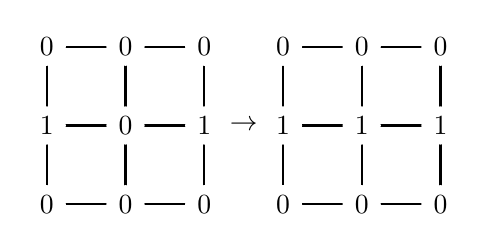
\begin{tikzpicture}
        % row1
        \cell{0}{0}{1}{1}
        \cell{1}{0}{2}{1}
        % row2
        \cell{0}{1}{1}{2}
        \cell{1}{1}{2}{2}
        % label for row1
        \( \lablvertex{0}{0}{$0$} \)
        \( \lablvertex{1}{0}{$0$} \)
        \( \lablvertex{2}{0}{$0$} \)
        % label for row2
        \( \lablvertex{0}{1}{$1$} \)
        \( \lablvertex{1}{1}{$0$} \)
        \( \lablvertex{2}{1}{$1$} \)
        % label for row3
        \( \lablvertex{0}{2}{$0$} \)
        \( \lablvertex{1}{2}{$0$} \)
        \( \lablvertex{2}{2}{$0$} \)
        
        % row1
        \cell{3}{0}{4}{1}
        \cell{4}{0}{5}{1}
        % row2
        \cell{3}{1}{4}{2}
        \cell{4}{1}{5}{2}
        % label for row1
        \( \lablvertex{3}{0}{$0$} \)
        \( \lablvertex{4}{0}{$0$} \)
        \( \lablvertex{5}{0}{$0$} \)
        % label for row2
        \( \lablvertex{3}{1}{$1$} \)
        \( \lablvertex{4}{1}{$1$} \)
        \( \lablvertex{5}{1}{$1$} \)
        % label for row3
        \( \lablvertex{3}{2}{$0$} \)
        \( \lablvertex{4}{2}{$0$} \)
        \( \lablvertex{5}{2}{$0$} \)

        \( \lablnode{2.5}{1}{$\rightarrow$} \)
    \end{tikzpicture}
\end{center}

The above transformation corresponds with \textit{either} two distinct polygons joining into one polygon \textit{or} one polygon splitting into two distinct polygons. In either case, we want the sign of the product to switch. This corresponds with the following constraint.

$$\text{sign}(w_{3}w_{2}w_{9}w_{5}) = -\text{sign}(w_{4}w_{4}w_{13}w_{13}).$$

All Type 1 constraints are as follows. For the following set of equations, assume the equals sign ($=$) means \textit{only} equal in sign.

\begin{eqnarray*}
    w_{1}w_{1}w_{2}w_{3} = w_{2}w_{3}w_{6}w_{11} & w_{1}w_{1}w_{2}w_{4} = w_{2}w_{3}w_{6}w_{12} & w_{1}w_{1}w_{4}w_{3} = w_{2}w_{3}w_{8}w_{11} \\
    w_{1}w_{1}w_{4}w_{4} = w_{2}w_{3}w_{8}w_{12} & w_{1}w_{2}w_{1}w_{5} = w_{2}w_{4}w_{5}w_{13} & w_{1}w_{2}w_{1}w_{6} = w_{2}w_{4}w_{5}w_{14} \\
    w_{1}w_{2}w_{2}w_{8} = w_{2}w_{4}w_{6}w_{16} & w_{1}w_{2}w_{4}w_{8} = w_{2}w_{4}w_{8}w_{16} & w_{3}w_{1}w_{9}w_{1} = w_{4}w_{3}w_{13}w_{9} \\
    w_{3}w_{1}w_{11}w_{1} = w_{4}w_{3}w_{15}w_{9} & w_{3}w_{1}w_{12}w_{3} = w_{4}w_{3}w_{16}w_{11} & w_{3}w_{1}w_{12}w_{4} = w_{4}w_{3}w_{16}w_{12} \\
    w_{3}w_{2}w_{12}w_{8} = w_{4}w_{4}w_{16}w_{16} & w_{1}w_{6}w_{1}w_{5} = w_{2}w_{8}w_{5}w_{13} & w_{1}w_{6}w_{1}w_{6} = w_{2}w_{8}w_{5}w_{14} \\
    w_{1}w_{6}w_{2}w_{8} = w_{2}w_{8}w_{6}w_{16} & w_{1}w_{6}w_{4}w_{8} = w_{2}w_{8}w_{8}w_{16} & w_{3}w_{6}w_{12}w_{8} = w_{4}w_{8}w_{16}w_{16} \\
    w_{5}w_{9}w_{1}w_{1} = w_{6}w_{11}w_{5}w_{9} & w_{5}w_{13}w_{1}w_{1} = w_{6}w_{15}w_{5}w_{9} & w_{5}w_{14}w_{1}w_{5} = w_{6}w_{16}w_{5}w_{13} \\
    w_{5}w_{14}w_{1}w_{6} = w_{6}w_{16}w_{5}w_{14} & w_{5}w_{14}w_{2}w_{8} = w_{6}w_{16}w_{6}w_{16} & w_{5}w_{14}w_{4}w_{8} = w_{6}w_{16}w_{8}w_{16} \\
    w_{11}w_{1}w_{9}w_{1} = w_{12}w_{3}w_{13}w_{9} & w_{11}w_{1}w_{11}w_{1} = w_{12}w_{3}w_{15}w_{9} & w_{11}w_{1}w_{12}w_{3} = w_{12}w_{3}w_{16}w_{11} \\
    w_{11}w_{1}w_{12}w_{4} = w_{12}w_{3}w_{16}w_{12} & w_{11}w_{2}w_{12}w_{8} = w_{12}w_{4}w_{16}w_{16} & w_{11}w_{6}w_{12}w_{8} = w_{12}w_{8}w_{16}w_{16} \\
    w_{13}w_{9}w_{1}w_{1} = w_{14}w_{11}w_{5}w_{9} & w_{15}w_{9}w_{9}w_{1} = w_{16}w_{11}w_{13}w_{9} & w_{15}w_{9}w_{11}w_{1} = w_{16}w_{11}w_{15}w_{9} \\
    w_{15}w_{9}w_{12}w_{3} = w_{16}w_{11}w_{16}w_{11} & w_{15}w_{9}w_{12}w_{4} = w_{16}w_{11}w_{16}w_{12} & w_{13}w_{13}w_{1}w_{1} = w_{14}w_{15}w_{5}w_{9} \\
    w_{13}w_{14}w_{1}w_{5} = w_{14}w_{16}w_{5}w_{13} & w_{13}w_{14}w_{1}w_{6} = w_{14}w_{16}w_{5}w_{14} & w_{13}w_{14}w_{2}w_{8} = w_{14}w_{16}w_{6}w_{16} \\
    w_{13}w_{14}w_{4}w_{8} = w_{14}w_{16}w_{8}w_{16} & w_{15}w_{13}w_{9}w_{1} = w_{16}w_{15}w_{13}w_{9} & w_{15}w_{13}w_{11}w_{1} = w_{16}w_{15}w_{15}w_{9} \\
    w_{15}w_{13}w_{12}w_{3} = w_{16}w_{15}w_{16}w_{11} & w_{15}w_{13}w_{12}w_{4} = w_{16}w_{15}w_{16}w_{12} & w_{15}w_{14}w_{9}w_{5} = w_{16}w_{16}w_{13}w_{13} \\
    w_{15}w_{14}w_{9}w_{6} = w_{16}w_{16}w_{13}w_{14} & w_{15}w_{14}w_{11}w_{5} = w_{16}w_{16}w_{15}w_{13} & w_{15}w_{14}w_{11}w_{6} = w_{16}w_{16}w_{15}w_{14} \\
\end{eqnarray*}

Similarly, all Type 2 constraints are as follows. Again, for the following set of equations, assume the equals sign ($=$) means \textit{only} equal in sign.

\begin{eqnarray*}
        -w_{3}w_{2}w_{9}w_{5} = w_{4}w_{4}w_{13}w_{13} & -w_{3}w_{2}w_{9}w_{6} = w_{4}w_{4}w_{13}w_{14} & -w_{3}w_{2}w_{11}w_{5} = w_{4}w_{4}w_{15}w_{13} \\
        -w_{3}w_{2}w_{11}w_{6} = w_{4}w_{4}w_{15}w_{14} & -w_{3}w_{6}w_{9}w_{5} = w_{4}w_{8}w_{13}w_{13} & -w_{3}w_{6}w_{9}w_{6} = w_{4}w_{8}w_{13}w_{14} \\
        -w_{3}w_{6}w_{11}w_{5} = w_{4}w_{8}w_{15}w_{13} & -w_{3}w_{6}w_{11}w_{6} = w_{4}w_{8}w_{15}w_{14} & -w_{5}w_{9}w_{2}w_{3} = w_{6}w_{11}w_{6}w_{11} \\
        -w_{5}w_{9}w_{2}w_{4} = w_{6}w_{11}w_{6}w_{12} & -w_{5}w_{9}w_{4}w_{3} = w_{6}w_{11}w_{8}w_{11} & -w_{5}w_{9}w_{4}w_{4} = w_{6}w_{11}w_{8}w_{12} \\
        -w_{5}w_{13}w_{2}w_{3} = w_{6}w_{15}w_{6}w_{11} & -w_{5}w_{13}w_{2}w_{4} = w_{6}w_{15}w_{6}w_{12} & -w_{5}w_{13}w_{4}w_{3} = w_{6}w_{15}w_{8}w_{11} \\
        -w_{5}w_{13}w_{4}w_{4} = w_{6}w_{15}w_{8}w_{12} & -w_{11}w_{2}w_{9}w_{5} = w_{12}w_{4}w_{13}w_{13} & -w_{11}w_{2}w_{9}w_{6} = w_{12}w_{4}w_{13}w_{14} \\
        -w_{11}w_{2}w_{11}w_{5} = w_{12}w_{4}w_{15}w_{13} & -w_{11}w_{2}w_{11}w_{6} = w_{12}w_{4}w_{15}w_{14} & -w_{11}w_{6}w_{9}w_{5} = w_{12}w_{8}w_{13}w_{13} \\
        -w_{11}w_{6}w_{9}w_{6} = w_{12}w_{8}w_{13}w_{14} & -w_{11}w_{6}w_{11}w_{5} = w_{12}w_{8}w_{15}w_{13} & -w_{11}w_{6}w_{11}w_{6} = w_{12}w_{8}w_{15}w_{14} \\
        -w_{13}w_{9}w_{2}w_{3} = w_{14}w_{11}w_{6}w_{11} & -w_{13}w_{9}w_{2}w_{4} = w_{14}w_{11}w_{6}w_{12} & -w_{13}w_{9}w_{4}w_{3} = w_{14}w_{11}w_{8}w_{11} \\
        -w_{13}w_{9}w_{4}w_{4} = w_{14}w_{11}w_{8}w_{12} & -w_{13}w_{13}w_{2}w_{3} = w_{14}w_{15}w_{6}w_{11} & -w_{13}w_{13}w_{2}w_{4} = w_{14}w_{15}w_{6}w_{12} \\
        -w_{13}w_{13}w_{4}w_{3} = w_{14}w_{15}w_{8}w_{11} & -w_{13}w_{13}w_{4}w_{4} = w_{14}w_{15}w_{8}w_{12} & 
\end{eqnarray*}

Solving all Type 1 and Type 2 constraints gives the following solution set.

\begin{center}
\begin{tabular}{|c|c|c|c|c|c|c|c|c|c|c|c|c|c|c|c|} 
\hline
$w_{1}$ & $w_{2}$ & $w_{3}$ & $w_{4}$ & $w_{5}$ & $w_{6}$ & $w_{7}$ & $w_{8}$ & $w_{9}$ & $w_{10}$ & $w_{11}$ & $w_{12}$ & $w_{13}$ & $w_{14}$ & $w_{15}$ & $w_{16}$ \\
\hline
7 & -1 & -1 & -1 & -1 & -1 & 0 & -1 & 1 & 0 & -1 & -1 & -1 & -1 & 1 & 7 \\
7 & -1 & -1 & -1 & -1 & 1 & 0 & 1 & 1 & 0 & 1 & 1 & -1 & 1 & -1 & 7 \\
7 & -1 & -1 & -1 & 1 & -1 & 0 & -1 & -1 & 0 & -1 & -1 & -1 & 1 & -1 & 7 \\
7 & -1 & -1 & -1 & 1 & 1 & 0 & 1 & -1 & 0 & 1 & 1 & -1 & -1 & 1 & 7 \\
7 & -1 & -1 & 1 & -1 & -1 & 0 & 1 & 1 & 0 & -1 & 1 & 1 & 1 & -1 & 7 \\
7 & -1 & -1 & 1 & -1 & 1 & 0 & -1 & 1 & 0 & 1 & -1 & 1 & -1 & 1 & 7 \\
7 & -1 & -1 & 1 & 1 & -1 & 0 & 1 & -1 & 0 & -1 & 1 & 1 & -1 & 1 & 7 \\
7 & -1 & -1 & 1 & 1 & 1 & 0 & -1 & -1 & 0 & 1 & -1 & 1 & 1 & -1 & 7 \\
7 & -1 & 1 & -1 & -1 & -1 & 0 & -1 & -1 & 0 & -1 & 1 & -1 & -1 & -1 & 7 \\
7 & -1 & 1 & -1 & -1 & 1 & 0 & 1 & -1 & 0 & 1 & -1 & -1 & 1 & 1 & 7 \\
7 & -1 & 1 & -1 & 1 & -1 & 0 & -1 & 1 & 0 & -1 & 1 & -1 & 1 & 1 & 7 \\
7 & -1 & 1 & -1 & 1 & 1 & 0 & 1 & 1 & 0 & 1 & -1 & -1 & -1 & -1 & 7 \\
7 & -1 & 1 & 1 & -1 & -1 & 0 & 1 & -1 & 0 & -1 & -1 & 1 & 1 & 1 & 7 \\
7 & -1 & 1 & 1 & -1 & 1 & 0 & -1 & -1 & 0 & 1 & 1 & 1 & -1 & -1 & 7 \\
7 & -1 & 1 & 1 & 1 & -1 & 0 & 1 & 1 & 0 & -1 & -1 & 1 & -1 & -1 & 7 \\
7 & -1 & 1 & 1 & 1 & 1 & 0 & -1 & 1 & 0 & 1 & 1 & 1 & 1 & 1 & 7 \\
7 & 1 & -1 & -1 & -1 & -1 & 0 & 1 & -1 & 0 & -1 & -1 & -1 & -1 & -1 & 7 \\
7 & 1 & -1 & -1 & -1 & 1 & 0 & -1 & -1 & 0 & 1 & 1 & -1 & 1 & 1 & 7 \\
7 & 1 & -1 & -1 & 1 & -1 & 0 & 1 & 1 & 0 & -1 & -1 & -1 & 1 & 1 & 7 \\
7 & 1 & -1 & -1 & 1 & 1 & 0 & -1 & 1 & 0 & 1 & 1 & -1 & -1 & -1 & 7 \\
7 & 1 & -1 & 1 & -1 & -1 & 0 & -1 & -1 & 0 & -1 & 1 & 1 & 1 & 1 & 7 \\
7 & 1 & -1 & 1 & -1 & 1 & 0 & 1 & -1 & 0 & 1 & -1 & 1 & -1 & -1 & 7 \\
7 & 1 & -1 & 1 & 1 & -1 & 0 & -1 & 1 & 0 & -1 & 1 & 1 & -1 & -1 & 7 \\
7 & 1 & -1 & 1 & 1 & 1 & 0 & 1 & 1 & 0 & 1 & -1 & 1 & 1 & 1 & 7 \\
7 & 1 & 1 & -1 & -1 & -1 & 0 & 1 & 1 & 0 & -1 & 1 & -1 & -1 & 1 & 7 \\
7 & 1 & 1 & -1 & -1 & 1 & 0 & -1 & 1 & 0 & 1 & -1 & -1 & 1 & -1 & 7 \\
7 & 1 & 1 & -1 & 1 & -1 & 0 & 1 & -1 & 0 & -1 & 1 & -1 & 1 & -1 & 7 \\
7 & 1 & 1 & -1 & 1 & 1 & 0 & -1 & -1 & 0 & 1 & -1 & -1 & -1 & 1 & 7 \\
7 & 1 & 1 & 1 & -1 & -1 & 0 & -1 & 1 & 0 & -1 & -1 & 1 & 1 & -1 & 7 \\
7 & 1 & 1 & 1 & -1 & 1 & 0 & 1 & 1 & 0 & 1 & 1 & 1 & -1 & 1 & 7 \\
7 & 1 & 1 & 1 & 1 & -1 & 0 & -1 & -1 & 0 & -1 & -1 & 1 & -1 & 1 & 7 \\
7 & 1 & 1 & 1 & 1 & 1 & 0 & 1 & -1 & 0 & 1 & 1 & 1 & 1 & -1 & 7 \\
\hline
\end{tabular}
\end{center}

Any of these assignments are sufficient for calculating $t_{m,n}$. 

\end{document}